%%%%%%%%%%%%%%%%%%%%%%% file template.tex %%%%%%%%%%%%%%%%%%%%%%%%%
%
% This is a general template file for the LaTeX package SVJour3
% for Springer journals.          Springer Heidelberg 2010/09/16
%
% Copy it to a new file with a new name and use it as the basis
% for your article. Delete % signs as needed.
%
% This template includes a few options for different layouts and
% content for various journals. Please consult a previous issue of
% your journal as needed.
%
%%%%%%%%%%%%%%%%%%%%%%%%%%%%%%%%%%%%%%%%%%%%%%%%%%%%%%%%%%%%%%%%%%%
%
% First comes an example EPS file -- just ignore it and
% proceed on the \documentclass line
% your LaTeX will extract the file if required
%
%\RequirePackage{fix-cm}
%
%\documentclass{svjour3}                     % onecolumn (standard format)
%\documentclass[smallcondensed]{svjour3}     % onecolumn (ditto)
%\documentclass[smallextended]{svjour3}       % onecolumn (second format)
%\documentclass[twocolumn]{svjour3}          % twocolumn
\documentclass[prodmode,acmjdiq]{acmsmall}


%%%\usepackage{graphicx}
\usepackage{breakcites}
%\usepackage{times}
\usepackage{ams}
%\usepackage{amsthm}
\usepackage{algo}
\usepackage{amsmath}
%\usepackage{appendix}
\usepackage{graphicx}
\usepackage{xspace}
\usepackage{color}
\usepackage{subfigure}
%\usepackage[small,compact]{titlesec}
%\usepackage{ulem} % Strikethrough font.
%\usepackage{abstract}
\usepackage[ruled,vlined]{algorithm2e}
%\usepackage[lined,boxed,commentsnumbered]{algorithm2e}
\usepackage{balance}
\usepackage[htt]{hyphenat}


% comments
\newcommand{\mike}[1]{{\textcolor{green}{#1 -- MJF}}}
\newcommand{\joe}[1]{{\textcolor{red}{#1 -- JMH}}}
\newcommand{\minos}[1]{{\textcolor{cyan}{#1 -- MG}}}
\newcommand{\daisy}[1]{{\textcolor{magenta}{#1 -- DZW}}}
\newcommand{\sean}[1]{{\textcolor{blue}{#1--SLG}}}

% CASTLE
\newcommand{\sysName}{pi\textsc{-CASTLE}\xspace}

% general
\renewcommand{\ttdefault}{cmtt}
\newcommand{\rbox}{\hfill $\Box$}

\newtheorem{thm}{Thorem}
\newtheorem{lem}{Lemma}
\newtheorem{ex}{Example}
\newtheorem{df}{Definition}[section]

\newcommand{\eat}[1]{}
\newcommand{\vpar}{\vspace*{.5em}}
\newcommand{\cut}[1]{}

\newenvironment{compactitemize}%
    {\begin{list}{}{
       \renewcommand{\makelabel}[1]{\bf $\bullet$}\hfil%
       \settowidth{\labelwidth}{\bf $\bullet$}%
       \setlength{\partopsep}{0mm}%
       \setlength{\parsep}{0mm}%
       \setlength{\parindent}{0mm}%
       \setlength{\itemsep}{0mm}%
       \setlength{\topsep}{0mm}%
       \setlength{\leftmargin}{\labelwidth}%
       \addtolength{\leftmargin}{\labelsep}
     }}%
    {\end{list}}

% BayesStore
\newcommand{\bs}{\textsc{BayesStore}\xspace}
\newcommand{\largebs}{{\large{\textsc{BayesStore}}}\xspace}
\newcommand{\Largebs}{{\Large{\textsc{BayesStore}}}\xspace}
\newcommand{\LARGEbs}{{\LARGE{\textsc{BayesStore}}}\xspace}
\newcommand{\hugebs}{{\huge{\textsc{BayesStore}}}\xspace}

% VLDB08 Abbreviations:
\newcommand{\ir}{$R$\xspace}
\newcommand{\sensor}{\textsl{Sensor1}\xspace}
\newcommand{\irset}{$\mathcal{R}$\xspace}
\newcommand{\pr}{\mbox{\sf Pr}}
\newcommand{\dom}{\mbox{\sf dom}}
\newcommand{\pdf}{$F$\xspace}
\newcommand{\true}{$true$\xspace}
\newcommand{\false}{$false$\xspace}
%\newcommand{\model}{$\mathcal{M}$}
\newcommand{\mv}{\textsl{miss}\xspace}
\newcommand{\RV}{\textsc{rv}\xspace}
\newcommand{\RVs}{\textsc{rv}s\xspace}
\newcommand{\bns}{\textsc{BN}s\xspace}
\newcommand{\mrfs}{\textsc{MRF}s\xspace}
\newcommand{\mrf}{\textsc{MRF}\xspace}
\newcommand{\rv}{$X$}
\newcommand{\pa}{$\mathcal{A}^p$\xspace}
\newcommand{\da}{$\mathcal{A}^d$\xspace}
\newcommand{\ed}{$\mathcal{ED}$}
%\newcommand{\entity}{e\xspace}
\newcommand{\es}{$\mathcal{E}$\xspace}
\newcommand{\op}{$\theta$\xspace}
%\newcommand{\bnf}{$\varphi$\xspace}
\newcommand{\fobnf}{$\phi$\xspace}
\newcommand{\fobn}{$\mathcal{M}_{FOBN}$\xspace}
\newcommand{\bn}{\textsc{bn}\xspace}
%\newcommand{\fbn}{$\textsc{fobn}$\xspace}
\newcommand{\MV}{$NULL$\xspace}
\newcommand{\mapping}{$f$\xspace}
\newcommand{\stripe}{$S$\xspace}
\newcommand{\selectivity}{\textsl{sel}\xspace}
\newcommand{\size}{\textsl{size}\xspace}
\newcommand{\missing}{\textsl{mratio}\xspace}
\newcommand{\connectivity}{\textsl{cratio}\xspace}
\newcommand{\probDB}{$\mathcal{DB}^p$}
%\newcommand{\exf}{$\mathcal{E}$}

% ICDE10

\newcommand{\tf}{text-string\xspace}
\newcommand{\IPD}{IPS\xspace}
\newcommand{\tfs}{text-strings\xspace}
\newcommand{\Tfs}{Text-strings\xspace}
\newcommand{\ie}{\textsc{ie}\xspace}
\newcommand{\model}{$\mathcal{M}$\xspace}
\newcommand{\tokenset}{\ensuremath{\mathbf{X}}\xspace}
\newcommand{\tokenseq}{\ensuremath{\mathbf{x}}\xspace}
\newcommand{\rvset}{\ensuremath{\mathbf{V}}\xspace}
\newcommand{\token}{\ensuremath{x}\xspace}
\newcommand{\labelset}{\ensuremath{\mathbf{Y}}\xspace}
\newcommand{\labelseq}{\ensuremath{\mathbf{y}}\xspace}
\newcommand{\crf}{$\mathcal{M}_{CRF}$\xspace}
\newcommand{\tokentbl}{\textsc{TokenTbl}\xspace}
\newcommand{\mr}{\textsc{MR}\xspace}
\newcommand{\strs}{$\mathcal{D}$\xspace}
\newcommand{\str}{\textit{d}\xspace}
\newcommand{\probsel}{\textit{probsel}\xspace}
\newcommand{\pwd}{\textit{pwd$(D^p)$}\xspace}

% HFGM-286report

\newcommand{\hfgm}{\textsc{hfgm}\xspace}
\newcommand{\rvs}{\textsc{rv}s\xspace}
\newcommand{\prm}{\textsc{prm}\xspace}

% extensibility

\newcommand{\pgm}{\textsc{PGM}\xspace}
\newcommand{\fctrset}{$\mathcal{F}$\xspace}
\newcommand{\probdbms}{\textsc{PDBMS}\xspace}

\newcommand{\argmax}{\operatornamewithlimits{argmax}}


\usepackage[ruled]{algorithm2e}
\renewcommand{\algorithmcfname}{ALGORITHM}
\SetAlFnt{\small}
\SetAlCapFnt{\small}
\SetAlCapNameFnt{\small}
\SetAlCapHSkip{0pt}
\IncMargin{-\parindent}

%
% FIXME remove?
%\smartqed  % flush right qed marks, e.g. at end of proof
%

% Metadata Information
\acmVolume{0}
\acmNumber{0}
\acmArticle{0}
\acmYear{2015}
\acmMonth{0}

\doi{0000001.0000001}
\issn{1234-56789}


\begin{document}

\markboth{S. Goldbarg et al.}{A Probabilistically Integrated System for Crowd-Assisted Text Labeling and Extraction}

\title{A Probabilistically Integrated System for Crowd-Assisted Text Labeling and Extraction}

%\subtitle{Do you have a subtitle?\\ If so, write it here}

%\titlerunning{Short form of title}        % if too long for running head

\author{SEAN GOLDBERG
\affil{University of Florida}
DAISY ZHE WANG
\affil{University of Florida}
CHRISTAN GRANT
\affil{Brown University}
}

%\authorrunning{Short form of author list} % if too long for running head


%\date{Received: date / Accepted: date}
% The correct dates will be entered by the editor

%\titlerunning{pi-Castle}

\begin{abstract}
The amount of text data has been growing exponentially in recent
years.
State-of-the-art statistical text extraction methods over this data are
likely to contain errors.
Recent work has shown probabilistic databases
can store and query uncertainty over extraction results, however, these systems
do not nately result in a reduction of error.
In this paper we propose \sysName, a system that uses a probabilistic
database as an anchor to execute, optimize and integrate machine and human
computing.  Uncertain fields are crowdsourced with the goal of reducing
uncertainty and improving accuracy.  We use information theory to optimize the
set of questions and a novel Bayesian probabilistic model to integrate
uncertain crowd answers back into the database.  Experiments show promising
results in significantly reducing machine error using very small amounts of
data.  Additionally, probabilistic integration is shown to more effectively
resolve conflicting crowd answers and provide users with the flexibility to
tune the desired trade-off between accuracy and recall according to the need of
applications.
Using crowds to assist machine-learned models proves to be a cost-effective way to
close the ``last mile'' in terms of accuracy for text labeling and
extraction tasks.

\eat{The need to automatically process and store large amounts of
uncertain and imprecise machine learned data has necessitated the
use of Probabilistic Databases (PDBs) which maintain and allow
queries that carry a degree of uncertainty. Another emerging trend
is crowdsourcing incomplete data through frameworks such as Amazon
Mechanical Turk.  In this paper, we introduce \sysName, an uncertain
data management system for sequential labeling of automatically
extracted text data. \sysName is a complete system that blends
uncertainty management with crowdsourcing techniques designed to
clean the data and reduce overall uncertainty.  It represents a
merging of machine and human computation for efficient task
solutions balancing speed, cost, and accuracy.  Work presented here
is applied on automatic bibliographic citation labeling, though the
techniques laid out may be applied in numerous other information
extraction domains.\dzw{need to rewrite}}
\end{abstract}




% Via http://dl.acm.org/ccs.cfm 
\begin{CCSXML}
<ccs2012>
<concept>
<concept_id>10002951.10003260.10003282.10003296</concept_id>
<concept_desc>Information systems~Crowdsourcing</concept_desc>
<concept_significance>500</concept_significance>
</concept>
<concept>
<concept_id>10002951.10003317.10003347.10003352</concept_id>
<concept_desc>Information systems~Information extraction</concept_desc>
<concept_significance>500</concept_significance>
</concept>
</ccs2012>
\end{CCSXML}

\ccsdesc[500]{Information systems~Crowdsourcing}
\ccsdesc[500]{Information systems~Information extraction}

\keywords{Crowdsourcing, Information Extraction, Probabilistic Models}

\acmformat{Sean Goldberg, Daisy Zhe Wang, and Tim Kraska, 2015. A Probabilistically Integrated System for Crowd-Assisted Text Labeling and Extraction.}

\begin{bottomstuff}
This work was sponsored by many different people FIXME.

Author's addresses: S. Goldberg {and} D. Z. Wang {and} C. Grant,
Computer \& Information Science \& Engineering Department, University of Florida;
E457 CSE Building, PO Box 116120, Gainesville, Florida 32611-6120.

Emails: seanlgoldberg@gmail.com; daisyw@cise.ufl.edu, cgrant@cise.ufl.edu
\end{bottomstuff}

\maketitle


\section{Introduction}

% big text data, introduce text labeling and extraction
In recent years, there has been an explosion of unstructured text data in
social networks like Twitter and Facebook, in enterprises via emails and
digitized documents, and on the Web.
Automatic information extraction (IE) over large amounts of text is important
for applications that depend on efficient search and analysis, such as
question answering, trend analysis, and opinion mining.
Various types of structured information that can be extracted
include part-of-speech labels from tweets, named entities from emails, and
relational attributes from bibliography citations.

% current IE approach and chance for errors
The state-of-the-art approach for IE uses statistical machine learning (SML)
models and algorithms such as hidden Markov models (HMM) and conditional random
fields (CRF)~\cite{DBLP:conf/icml/LaffertyMP01}.  Most current IE systems
store the maximum likelihood extraction into a database for querying, but such
extractions using even the best models are still prone to errors even for a
task as simple as text segmentation. Consider the following example citations.
%\vspace{-1mm}
\begin{example}
\label{ex:citation} 
\begin{sloppypar}
\vspace{2mm} 
\noindent \texttt{Building New Tools for Synthetic Image 
Animation by Using Evolutionary Techniques Xavier 
Provot, David Crochemore, Michael Boccara, Jean
Louchet Artificial Evolution 3-540-61108-8 Springer} 
\vspace{2mm}
\end{sloppypar}
\noindent \textit{With no obvious distinction between fields, the model may mislabel \texttt{Xavier} as part of the \texttt{title} rather than \texttt{author}.
The model may also confuse treat \texttt{Artificial Evolution} as a \emph{journal} attribute or as the last \emph{author} attribute.}
\rbox
\end{example}
%\vspace{-2mm}

A possible means of correcting errors and improving the accuracy of SML-based
extraction results uses a human-in-the-loop, manually validating extractions
that the machine performs poorly on or is highly uncertain of.  When the
corrected extractions are re-introduced into the training set, this is known as
\textit{active learning}.
Human annotation is expensive and time-consuming.  Platforms like Amazon
Mechanical Turk (AMT) deploy Human Intelligence Tasks (HITs) that make it
possible to include humans as a resource during the text
extraction process in a \textit{convenient}, \textit{timely}, and
\textit{scalable} fashion.  An ideal IE system would be one that efficiently
leverages the advantages of both human and machine computation
\cite{DBLP:journals/pvldb/WangKFF12,quinn10} into a single cohesive unit.


%Most SML models can generate probability distributions that quantify its confidence over possible extractions, however, such uncertainty that could be used to identify possible errors is lost before entering a database. Recent work~\cite{Gupta:2006:CPD:1182635.1164210,DBLP:journals/pvldb/WangFGH10,DBLP:journals/pvldb/WickMM10,Wang11} shows the development of probabilistic databases that can store and query uncertainty in addition to the top-1 IE results.


%In order to correct errors and improve the accuracy of SML-based extraction results to near-perfect, human assistance is needed.  This can be seen as a data cleaning problem over SML results in the ``last mile''. Humans, compared to their electronic counterparts, are able to recognize context and draw upon a wealth of previous experience to achieve better accuracy for many text extraction tasks. For example, a human can easily recognize \emph{Xavier Provot} as an \emph{author}, and \emph{Artificial Evolution} as the a \emph{journal} in Example~\ref{ex:citation}.

%Platforms like Amazon Mechanical Turk (AMT) deploy Human Intelligence Tasks (HITs) that make it possible for the first time to include humans as a resource during the text extraction process in a convenient, timely, and scalable fashion. While crowdsourcing is in general more accurate, it is still far more expensive and slow than automated techniques. An ideal IE system would efficiently leverage the advantages of both human and machine computation~\cite{DBLP:journals/pvldb/WangKFF12,quinn10}.

For this purpose, we introduce \sysName: a crowd-assisted SML-based IE system. \sysName uses a probabilistic database to execute, optimize, and integrate human and machine computation for improving text extraction.  The human computation aspect is powered by (AMT) and the machine computation using linear-chain CRF models.  \sysName initially employs a CRF to annotate all input text data. In contrast to other IE systems, however, \sysName uses a probabilistic data model to store IE results and manage data cleaning.  It has the ability to automatically query humans to correct the most uncertain tokens and integrates their responses back into the data model.

By allowing machines to do most of the work and focusing on humans only in the ``last mile'', \sysName achieves an optimal balance
between cost, speed, and accuracy for IE problems. We address three challenges in the design and implementation of \sysName: the probabilistic data model, selection of uncertain entries, and integration of human corrections.

First, in order to utilize human computing to reduce errors and uncertainty in SML-based IE results, a probabilistic data model and system is needed to store the uncertain results as well as evidence obtained from the crowd.  We use the model described in~\cite{DBLP:conf/icde/WangMFGH10}, storing both uncertain relations and probabilistic models as first class objects.  We also implement a number of user defined functions (UDFs) for statistical inference, question selection, and uncertain data integration over this probabilistic data model to connect the SML and crowd components in \sysName.

%Second, AMT questions should be automatically generated from uncertain IE results and optimized to reduce the maximum amount of errors and uncertainty given a fixed budget. Not all questions are equally informative and we use information theory over the extraction uncertainty to guide the selection of questions.  Some questions can correct multiple errors through a combination of the dependence properties of the CRF and an application to multiple redundant entries in the database.   We apply a specific set of clustering and ranking functions to optimize our information theoretic selection algorithm.

The data cleaning process entails automatically selecting entries likely to be incorrect and generating questions to be pushed to AMT.  \sysName utilizes concepts from information theory such as mutual information to select the most informative entries.  This idea of informativeness is defined as those entries likely to reduce the maximum amount of error and uncertainty over the entire database.  This is a technically challenging task as tokens, represented as nodes in a graphical model, are not independent, but adhere to the dependence properties modeled by the CRF.  Correcting individual tokens can influence other surrounding tokens in the same neighborhood and \sysName takes this information into account.  Additionally, token redundancy across the database is used to make the most impactful corrections.

Lastly, answers from crowdsourcing services, while generally more accurate, can still contain erroneous and conflicting information if worker qualities are low or if questions are difficult or ambiguous. One of the standard techniques is to take a majority vote among a collection of workers, but such a deterministic approach does not capture the controversy and uncertainty in crowdsourced answers. We introduce a Bayesian probabilistic integration model for combining uncertain answers. This model uses prior knowledge to estimate the confidence of Turker answers and integrate uncertain and conflicting answers in a principled manner.  

%The last challenge is how to effectively integrate responses from AMT back into the database.  Crowdsourcing services, while in general more accurate than automatic processing, can still contain erroaneous and conflicting information if worker qualities are low or if questions are difficult or ambiguous.  \sysName implements a number of standard quality control mechanisms, but whereas most methods seek only to extract the maximum likelihood label, \sysName uses a Bayesian probabilistic combination model to obtain an accurate human-provided label distribution.  Crowd responses are integrated back into the database by constraining CRF nodes to this distribution before performing inference.

% contribution summary
The following are the key technical contributions of this paper:
\begin{compactitemize}
\item We design and implement a crowd-assisted IE system \sysName based on a CRF that uses a probabilistic database as an foundation to execute, optimize, and tightly integrate machine computation over CRF models and human computation over crowdsourcing services;
\item We develop novel information theoretic techniques that can automatically generate AMT questions to maximally reduce uncertainty and errors in IE result by as much as $60\%$. Using data from DBLP and PubMed repositories, we show that these techniques lead to orders-of-magnitude fewer questions, reducing cost in improving the overall accuracy of extractions;
\item We develop, implement and evaluate a Bayesian probabilistic combination model to integrate the uncertain data from multiple workers. Probabilistic integration of crowd answers can achieve up to $50\%$ over majority voting for relatively difficult questions. Additionally, such integration provides confidence values that can be used for accepting or rejecting a consensus answer.  The integrated probabilistic result gives the user the flexibility to tune the trade-off between accuracy and recall (as shown in Section~\ref{sec:experiments}) according to the need of the application.
\end{compactitemize}
\vspace{1mm}

The paper is summarized as follows.  Section~\ref{sec:background} covers the necessary background in probabilistic databases, conditional random fields, and Amazon Mechanical Turk.  We give an overview of the \sysName system in Section~\ref{sec:system}.  Sections~\ref{sec:selection} and~\ref{sec:integration} cover our techniques for performing question selection and integration respectively.  Our experiments can be found in Section~\ref{sec:experiments}, while Sections~\ref{sec:related} and~\ref{sec:conclusion} contain the Related Work and Conclusions.

\eat{
%1. Introduce problem of information extraction
%The web is becoming an ever increasing expanse of information and knowledge.  Unfortunately, the majority of this data is not easily manipulated or analyzed by computers.  Granting structure to the trove of unstructured data for storage in a database is the key to efficient and complex searching, querying, and analysis. Traditionally it's been the job of humans to provide such metadata and structure, filling out the database by hand, but this is typically a slow and expensive process.  Information extraction is the method of performing this annotation automatically and at scale, rapidly increasing speed and dramatically lowering costs.

%Applications of information extraction include part-of-speech tagging \cite{DBLP:conf/acl/Ratnaparkhi98}, shallow parsing \cite{DBLP:conf/naacl/ShaP03}, named entity recognition \cite{DBLP:conf/cikm/Zhang04}, contact information extraction \cite{DBLP:conf/aaai/KristjanssonCVM04}, and bibliographic information extraction \cite{Wellner2004}.  One of the leading automated techniques employs the use of linear-chain conditional random fields (CRFs) \cite{DBLP:conf/icml/LaffertyMP01}, a generalization of Hidden Markov Models, for sequential tagging. Even the most state-of-the-art automated models are error-prone, however, and suffer from a lack of true contextual recognition and a lack of training data to cover the entire domain.

%\eat{ Recognizing certain fields such as the title or author are simple tasks for most individuals, but represents a challenging problem for machines.    CRFs can also perform tasks such as part-of-speech annotation \cite{}XXXX and named entity recognition.

%Automated processing of these tasks is a difficult proposition as evinced by the following bibliographic information extraction example.}

%2. Introduce subset of text segmentation
\begin{example}
\label{ex:citation}
Consider the following example scientific citation:

\vspace{5mm}
\parbox{.45\textwidth}{\textit{Building New Tools for Synthetic Image Animation by Using Evolutionary Techniques. Xavier Provot, David Crochemore, Michael Boccara, Jean Louchet Artificial Evolution 3-540-61108-8 Springer Lecture Notes in Computer Science Artificial Evolution, European Conference, AE 95, Brest, France, September 4-6, 1995, Selected Papers 1996}}
\vspace{5mm}

Even without punctuation in some locations, we are able to
differentiate tokens into their respective fields.  A machine may
not intuitively recognize 'Michael' or 'Jean' as being names and
certainly doesn't understand the concept of 'Artificial Evolution'
and why it's highly unlikely to be an author name.
\end{example}

%4. Problem: even the best machine results introduce some error
Humans, compared to their mechanical counterparts, are able to
recognize context and draw upon a wealth of previous experience that
computers cannot compare with.   There is a well known tradeoff
\cite{Quinn10crowdflow:integrating} between the level of accuracy
achieved by human processing and the speed and financial gains from
machine processing.

%5. Introduce crowdsourcing
Recently there has been increasing development of ''human computation
marketplaces'' such as Amazon Mechanical Turk
\cite{Ipeirotis:2010:AAM:1869086.1869094}.  Developing microtasks
that can be distributed concurrently to thousands of people at once
at reduced cost has greatly increased the utility of hiring human
workers to do trivial tasks such as annotation, ranking, and
searching on the internet.  While significantly cheaper than hiring
human experts, the cost of crowdsourcing is still much greater than
processing a task using automated techniques.  The ideal scenario
would leverage the advantages of both human and machine computation
efficiently.

We propose the Crowd-Assisted Machine Learning, or CAMeL, a paradigm
for the merging of human and machine intelligence.  Automated
machine learning is run first over a task before crowdsourcing is
used to clean up and improve elements of the output that are most
uncertain.  Many of the core elements introduced throughout this
paper such as uncertainty management and data integration are
applicable to a wide range of machine learning tasks utilizing text,
images, and speech.  As a starting point, we choose to focus on
textual annotation here and leave additional tasks as future work.

Thus we are led to introduce \sysName, a probabilistic database
augmented with crowdsourcing, designed to take advantage of the
strengths of human and machine computation in a unified manner for
the purpose of textual labeling and extraction.  After a CRF model
is used to initially annotate the data, humans are introduced to
correct the most uncertain tokens.  Our specific notion of
uncertainty is defined and expanded upon in Section
~\ref{sec:selection}.  By allowing machines to do most of the work
and focusing on humans only in the "last mile", \sysName is able to
achieve an optimal balance between cost, speed, and accuracy in
solving information extraction problems.  The same is true of any
future system using the CAMeL paradigm.

There are many challenges which need to be met in designing a system
such as \sysName .  First, uncertainty needs to managed and
maintained at all stages.  Second, questions about uncertain fields
posed to the crowd should be minimized given a fixed cost.  Lastly,
quality should be upheld even when dealing with a possibly noisy
and/or conflicting crowd.

Uncertainty is inherent in the construction of any system that
operates over statistical machine learning.  Probabilistic base
tables allow for a representation of multiple \textit{possible
worlds} with varying probabilities and manipulations of the data
behave according to their underlying distributions.  There is a
philosophical reflection to be had in the treatment of data this
way.  Decisions about the structure of data are always inferred,
never truthed, and incoming evidence, be it from additional learning
algorithms, human experts, or crowdsourced responses, always has the
ability to update these decision processes.

For the second challenge, only posing questions to the crowd for
which there is a reasonable enough assumption of incorrectness can
drastically reduce costs and allow those examples "easy enough" to
be done by mechanical methods to be done swiftly and cheaply.
\sysName uses information theory in a manner similar to uncertainty
sampling in active learning for this selection process.  It also has
the power to recognize redundancy and map multiple fields into a
single question.

The final challenge for a system like \sysName and greatest
difficulty for integrating a crowd of non-experts is the noisiness
of the response.  The economics of the Amazon Mechanical Turk
marketplace provide little incentive for a worker to submit high
quality work and weeding out the response of lazy and malicious
workers is an area of active research in the crowdsourcing
community.  One of the standard techniques is to take a majority
vote among a collection of workers, but such a deterministic
approach can be untrustworthy if all workers are of low quality and
removes information about possible controversy or conflict from
challenging questions.  This added information is useful in deciding
whether to trust the crowd's decision.  Since \sysName is a
probabilistic database, we introduce Bayesian and Dempster-Shafer
approaches to integrate responses probabilistically.  As far we
know, we are the first to pursue such an integration among crowd
responses.

\sysName makes a number of contributions to the burgeoning field of probabilistic data management.
\begin{itemize}
\item Probabilistic base tables are used to store the uncertainty in both the ML extracted results and human contributions.
\item A novel technique that clusters fields and ranks by entropy ensures question results carry a large degree of information back into the system.  We show that compared to a random baseline our method is able to reduce the number of questions given a fixed budget by an order of magnitude.
\item For integration of uncertain crowd results, we propose two methods based on a Bayesian framework and Dempster-Shafer belief theory that differ primarily in their initial prior distributions.  In addition to being more informative on the confidence of answers, both probabilistic integration methods achieved a gain of 7\% in accuracy over their deterministic counterpart, majority voting.
\end{itemize}

The driving application we investigate throughout the paper is
bibliographic citation information extraction as per
Example~\ref{ex:citation}.  The explicit task for both the machine
and humans given a token from from a citation document is to label
the appropriate field that token belongs to, eg., Title, Author,
Journal, etc.  This is only one application instance and the
\sysName system can be applied to any textual annotation task such
as named entity recognition or relationship extraction.

This paper is organized as follows.  We discuss necessary background
information in Section~\ref{sec:background}.
Section~\ref{sec:system} overviews of the system components and
their interactions.  Selection and clustering of fields for question
minimization is discussed in Section~\ref{sec:selection}.  Our
approach to probabilistic integration is presented in
Section~\ref{sec:integration}, while Section~\ref{sec:experiments}
contains experimental results.  Related work is in
Section~\ref{sec:related}.  Finally, Sections~\ref{sec:conclusion}
and~\ref{sec:future} contain the conclusion and our future work,
respectively. }


\section{Background}
\label{sec:background}

In this section we briefly describe the necessary background to understanding key components of the \sysName system.
\subsection{Probabilistic Databases}

A \textit{probabilistic database} $\mathcal{DB}^{p}$ consists of two key components: (1) a collection of incomplete relations $\mathcal{R}$ with missing or uncertain data, and (2) a probability distribution $F$ on all possible database instances.  These \textit{possible worlds} denoted by pwd($DB^{p}$) represent multiple viable instances of the database.  The attributes of an incomplete relation $R \in \mathcal{R}$ may contain deterministic attributes, but also include a subset that are \textit{probabilistic attributes} $\mathcal{A}^{p}$.  The values of $\mathcal{A}^{p}$ may be present, missing, or uncertain.  Each possible database instance is a completion of the missing or uncertain data in $\mathcal{R}$.

\subsection{Conditional Random Fields (CRF)}
\label{sec:pi-crf}
\begin{figure}
        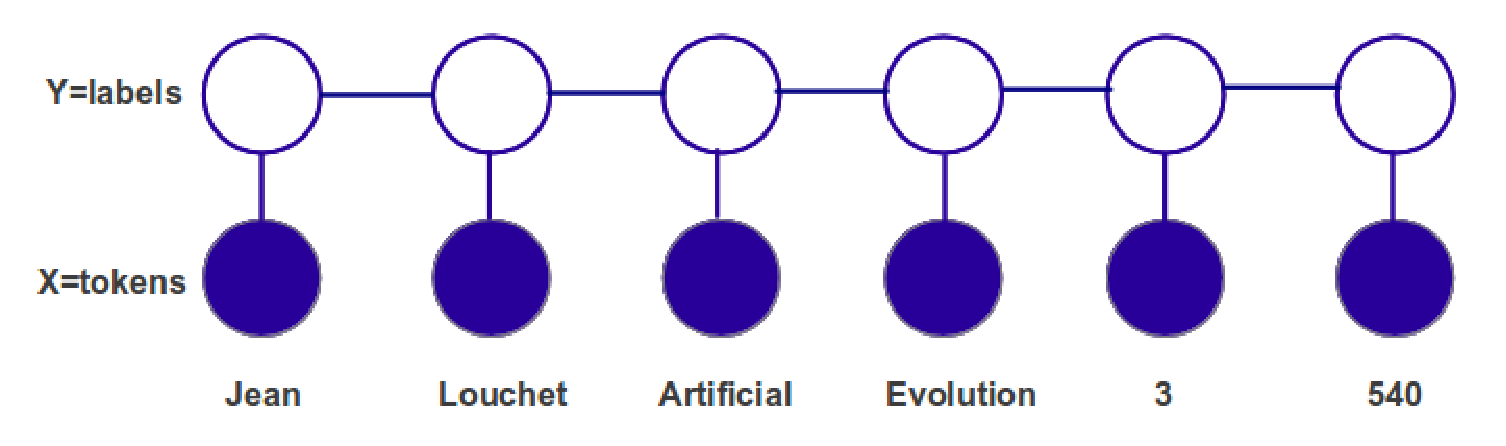
\includegraphics[width=0.9\textwidth]{CRF.eps}
        \caption{Example CRF model.}
        \label{fig:CRF}
\end{figure}

The linear-chain CRF~\cite{DBLP:conf/icml/LaffertyMP01,sutton06introduction}, an extension of the hidden Markov model, is a state-of-the-art probabilistic graphical model for solving IE tasks.  In the context of IE, a CRF model encodes the probability distribution over a set of \textit{label} random variables $y \in \mathbf{Y}$, given the value of a set of \textit{token} random variable $x \in \mathbf{X}$.  Assignments to $\mathbf{X}$ are given by $\mathbf{x}$ and to $\mathbf{Y}$ by $\mathbf{y}$.  In a linear-chain CRF model, label $y_{i}$ is correlated only with the previous label $y_{i-1}$ and the corresponding token $x_{i}$.  The set of these correlations $k \in K$ are represented by the feature functions $\{f_{k}(y_{i},y_{i-1},x_{i})\}^{K}_{k=1}$.

\begin{example}
Figure~\ref{fig:CRF} shows an example CRF model over a subset of the citation string from Example~\ref{ex:citation}.  Observed (known token) variables are shaded nodes in the graph.  Hidden (unknown label) variables are unshaded.  Edges in the graph denote statistical correlations.  For citations, the possible labels are $Y = \{$title, author, conference, isbn, publisher, series, proceedings, year\}.  Two possible feature functions of this CRF are:
\begin{align*}
    \centering
    f_{1}(y_{i}, y_{i-1}, x_{i}) &= [x_{i} \text{ appears in a conf list}] \cdot [y_{i} = \text{ conf}]\\
    f_{1}(y_{i}, y_{i-1}, x_{i}) &= [y_{i} = \text{ author}] \cdot [y_{i-1} = \text{ title}]
\end{align*}
\end{example}
Let $\{f_{k}(y_{i},y_{i-1},x_{i})\}^{K}_{k=1}$ be a set of real-valued feature functions, and $\Lambda = \{\lambda_{k}\} \in R^{K}$ be a vector of real-valued parameters, a CRF model defines the probabilistic distribution of segmentations $\mathbf{y}$ given a specific token sequence $\mathbf{x}$:
\begin{equation}
\label{eq:CRFmodel}
p(\mathbf{y} | \mathbf{x}) = \frac{1}{Z}\text{exp}\{\sum_{i=1}^{T}\sum_{k=1}^{K}\lambda_{k}f_{k}(y_{i},y_{i-1},x_{i})\},
\end{equation}
where $Z$ is a standard partition function that guarantees probability values between $0$ and $1$.

\subsection{Inference Queries over a CRF Model}
\newcommand{\topk}{top-\textit{k}\xspace}
There are three types of inference queries used in \sysName .

\textbf{Top-k Inference}: The \topk inference computes the segmentations with the \topk highest probabilities given a token sequence $\mathbf{x}$ from a text-string $d$.  The Viterbi dynamic programming algorithm~\cite{Viterbi1973} is the key algorithmic technique for CRF \topk inference.

%The Viterbi algorithm computes a two-dimensional V matrix, where each cell $V(i,y)$ stores a ranked list of \textit{entries} $e=\{score,$ $prev(label,idx)\}$ ordered by a \textit{score}.  Each entry contains (1) the \textit{score} of a \topk (partial) segmentation ending at position $i$ with label $y$; and (2) a pointer to the previous entry \textit{prev} on the path that led to the \topk \textit{score's} in $V(i,y)$.  The pointer $\text{e.prev}$ consists of the label $label$ and the list index $idx$ of the previous entry on the path to $e$.  Based on equation~\ref{eq:CRFmodel}, the recurrence to compute the ML (top-1) segmentation is as follows:
%\begin{equation}
%V(i,y) = \left\{
%\begin{array}{l l}
%\text{max}_{y'}(V(i-1,y')\\
%   + \sum_{k=1}^{K}\lambda_{k}f_{k}(y,y',x_{i})), & \quad \text{if } i \geq 0\\
%0, & \quad \text{if } $i$ = -1
%\end{array} \right.
%\end{equation}
%\eat{
%The ML segmentation $y*$, backtracked from the maximum entry in $V(T,y_{T})$ (where $T$ is the length of the token sequence \textbf{x}) through $\text{prev}$ pointers is shown in Figure~\ref{}.  }
%The complexity of the Viterbi algorithm is $O(T \cdot |L|^{2})$, where $|L|$ is the number of possible labels.

\textbf{Constrained Top-k Inference}: Constrained \topk inference~\cite{Kristjansson:2004:IIE:1597148.1597216} is a special case of traditional \topk inference.  It is used when a subset of the token labels has been provided (e.g., via a user interface such as Amazon Mechanical Turk).  Let $\mathbf{s}$ be the evidence vector $\{s_{1}, \dots, s_{T}\}$, where $s_{i}$ is either NULL (i.e., no evidence) or the evidence label for $y_{i}$.  Constrained \topk inference can be computed for a variant of the Viterbi algorithm which restricts the chosen labels $\mathbf{y}$ to conform to the evidence $\mathbf{s}$.

\textbf{Marginal Inference}: Marginal inference computes a marginal probability $p(y_{t},y_{t+1}, \dots, y_{t+k}|\mathbf{x})$ over a single node's label or a sub-sequence of nodes~\cite{sutton06introduction}.  The Forward-Backward algorithm, a variation of the Viterbi algorithm is used for such marginal inference tasks.  In \sysName, marginal inference is primarily employed over a single node corresponding to the marginal label distribution for individual tokens. 

%\subsection{Uncertainty Sampling}
%\label{sec:uncertainty}
%Uncertainty sampling has a long history in pool-based active learning~\cite{Lewis94heterogeneousuncertainty} and seeks to optimally select a set of unlabeled examples for labeling by experts.  The approach selects those that are the "least certain," which means they have the highest variance over their label distributions.  One method for quantifying uncertainty over a random variable \textbf{X} is through its entropy~\cite{cover91}:
%\begin{equation}
%H(\mathbf{X}) = \sum p_{i}(\mathbf{X})log(p_{i}(\mathbf{X})).
%\end{equation}
%Given sets of random variables $\mathbf{X}$ and $\mathbf{Y}$ with dependency properties (such as may be found in a sequence model like CRF), observing variables produces a conditional entropy
%\begin{equation}
%H(\mathbf{Y}|\mathbf{X}) = H(\mathbf{X},\mathbf{Y}) - H(\mathbf{X}).
%\end{equation}
%\eat{
\subsection{Crowdsourcing}

Platforms such as Amazon Mechanical Turk (AMT) and Crowdflower have made the leveraging of human computation and intelligence at large scale both cost effective and time efficient.  Workers, or``Turkers'', complete various jobs and earn money on a per-job basis.  The range of ``microtasks'' available for completion may be anything from simple image or text annotation tasks, completing surveys, or ranking search results, usually within a few minutes and at a cost of a few cents per task.  These jobs generally don't require any special training or domain expertise, allowing a large workforce from all over the world to be utilized.  Amazon does not publish current statistics about the marketplace, but it contained over 200,000 \cite{AWS:2006} Turkers in 2006, and by all estimates, has grown dramatically since then \cite{Ross:2010:CSD:1753846.1753873}.

\section{System Overview}
\label{sec:system}

\begin{figure}[t]
        \centering
        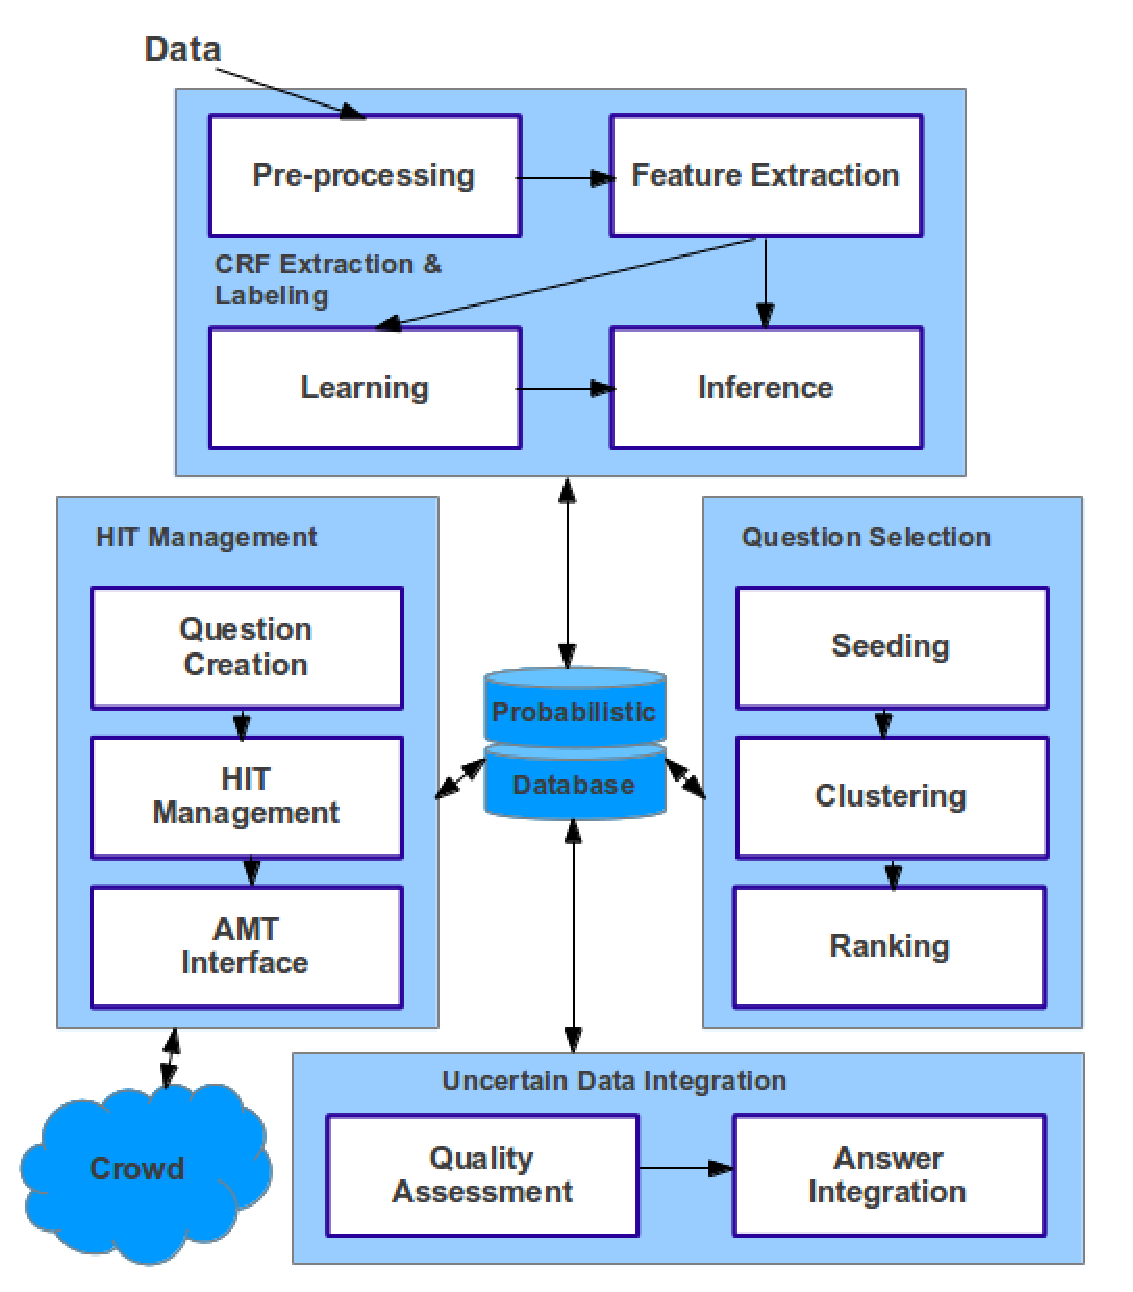
\includegraphics[width=.9\textwidth]{architecture.eps}
        \caption{Architecture of the \sysName system.}
        \label{fig:system}
\end{figure}

Figure~\ref{fig:system} outlines the basic architecture of the \sysName system, which is comprised of four main components: 1. CRF Extraction \& Inference, 2. Question Selection, 3. HIT Management, and 4. Uncertain Data Integration. The arrows chart the flow of data within and between different components. Overall, data flows through the four components in order. First, SML models are applied to perform automatic text extraction and labeling. The uncertain extractions are stored in a probabilistic database. Second, a set of ranked questions are selected from uncertain IE results. Third, the HIT manager formulates and pushes these questions to the crowd and retrieves the answers. Fourth, the Turker answers are combined probabilistically and integrated back into the database, improving the initial IE results from the CRF.

In this section we briefly outline each of the system's components and how they are related, as well as how data is specifically stored in the data model.
While we use existing techniques for 1. CRF Extraction and 3. HIT Management, we develop novel techniques for 2. Question Selection and 4. Uncertain Data Integration in Section~\ref{sec:selection} and Section~\ref{sec:integration}.

\subsection{Feature Extraction \& Inference}

The initial extraction and labeling of unstructured text is handled by the Extractor \& Inference module.  Parameter estimation
(learning) of the model is done in advance using a labeled data set. Maximum likelihood labels and marginal probabilities can be inferred from the CRF model and the uncertain label or extraction tables in a probabilistic database. We adopt the probabilistic data model outlined in~\cite{DBLP:journals/pvldb/WangFGH10}.

Unstructured text is treated as a set of documents or text-strings $\mathcal{D}$.  Each document $d \in \mathcal{D}$ has a substructure comprising a set of tokens $t^{d}_{i}$, where $i \in \{1, \dots, N\}$ and $N$ is the length of the string (document). These tokens are stored in the relational format with attributes (\emph{docID, pos, token}). In addition, a probabilistic attribute label$^{p}$ is also included, whose value can be inferred by the model. The schema of the uncertain IE results generated from the CRF is: \

\begin{figure*}[t]
        \centering
	\setlength\fboxsep{0pt}
	\setlength\fboxrule{0.5pt}
        \fbox{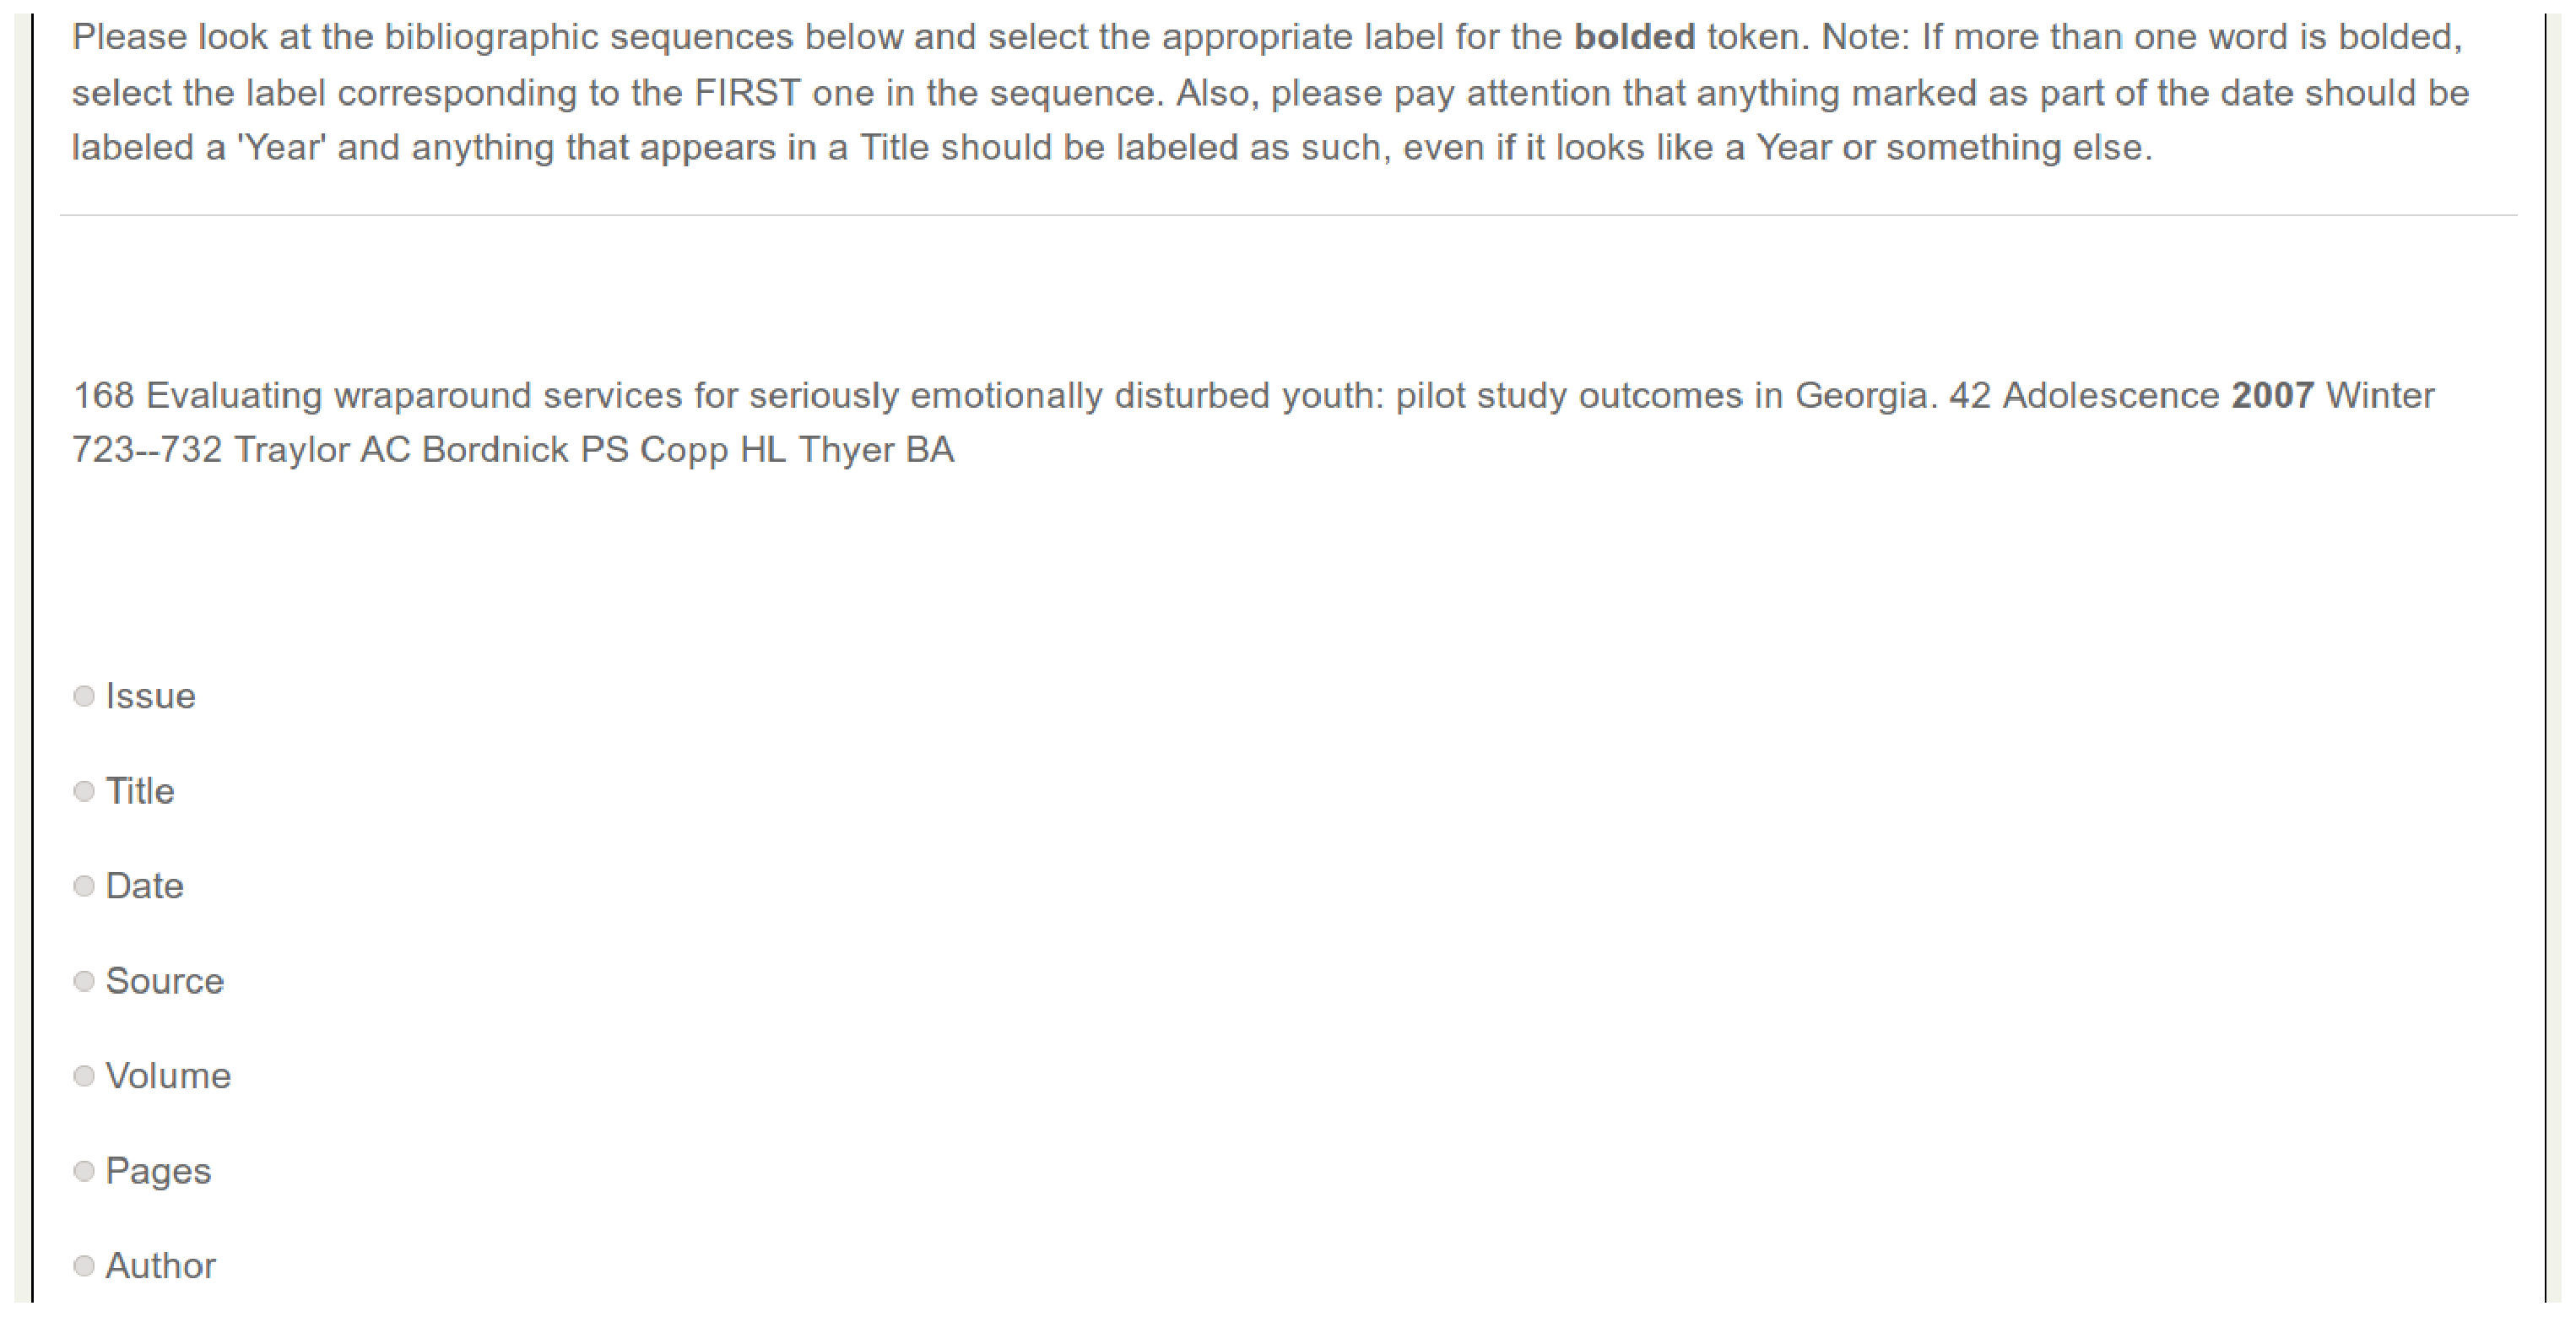
\includegraphics[width=.95\textwidth]{interface.eps}}
        \caption{Sample Mechanical Turk HIT Interface}
        \label{fig:HIT_int}
\end{figure*}

\vspace{.1in} \centerline{C{\small RF}L{\small BL}T{\small BL}(docID, pos, token, label$^{p}$)} \vspace{.1in}

The probabilistic label attribute label$^{p}$ maps to a random variable within a grounded CRF model.  Queries such as MARGINAL and TOP-K extraction can be run over the collection of probabilistic labels.

\subsection{Question Selection}

The novelty of \sysName is that it improves the results of automatic text labeling and extraction with additional evidence collected from the crowd.  Utilizing data uncertainty information, it automatically selects questions over tokens that are more uncertain and likely to contain errors. This process of \textit{Question Selection} is illustrated by the right-hand module in Figure~\ref{fig:system}, which applies three consecutive techniques over the uncertain C{\small RF}L{\small BL}T{\small BL} table: Filtering, Clustering, and Ranking. Filtering selects an initial set of tokens to be corrected based on mutual information; Clustering, groups those filtered tokens with similar attributes together using a trigram contextual model to reduce redundancy; Ranking, performs a total ordering over token clusters.  Cluster assignments and rankings for all tokens passing the initial Filtering operation are stored in a selection table.

\vspace{.1in} \centerline{S{\small ELECTION}T{\small BL} (docID, pos, clusterID, ranking)} \vspace{.1in}

The selection of questions is performed with a fixed budget and optimized for the cost of each question.
We focus on uniform, fixed-cost questions, though our methods may be easily extended to multiple question types incurring different costs.

%Assuming the labeling of a single token can be mapped to a single AMT question, \textit{seeding} generates the initial set of candidate tokens. These seeded tokens, if translated into questions and labeled by humans, would be more informative than the rest of the tokens. We use information theory and entropy to select this first batch of candidates. The selected tokens are then \textit{clustered} by similarity to find cases where a single question can resolve multiple errors or uncertainty. The intuition is that we should ask different enough questions to reduce the information overlap between questions. Finally, candidate tokens are ranked by the information gain, which is estimated by the token entropy and the token cluster. The \topk tokens selected are stored into a selection table.



\subsection{HIT Management}

The HIT manager has the responsibility of taking the rows of S{\small ELECTION}T{\small BL}, converting them into AMT questions (i.e., HITs), and posting those questions onto Amazon Mechanical Turk. The Question Creation subcomponent generates an XML template for a multiple choice question for each selected token. An example interface is shown in Figure~\ref{fig:HIT_int}. The entire text document (in this case a citation) is shown and the queried token is bolded.  Users select from the set of all labels the one they believe belongs to the bolded token. The Question Creator has the ability to assign multiple questions to a single HIT, this ensures Turkers answer the same subsets of questions.

The HIT manager also allows an administrator to set specifics such as the price of each HIT, length of posting, and the number of Turkers assigned to each HIT.  There is an AMT interface that uses an API to handle both the posting of questions and retrieval of answers. Both questions and answers are recorded and stored in their corresponding base tables, the primary key being a HITID supplied by Amazon when posting.

\vspace{.1in}
\centerline{P{\small OST}T{\small BL}(docID, pos, HITID)}
\vspace{.1in}

\centerline{T{\small URKER}L{\small BL}T{\small BL}(HITID, workerID, label)}
\vspace{.1in}

\subsection{Uncertain Data Integration}

The goal of integration in \sysName is to use both the crowd supplied labels and the machine generated labels to infer the annotation distribution. The first step is to assess the quality of each Turker using the well-documented method introduced by Dawid \& Skene~\cite{1979}.  This tells us how to appropriately weight Turkers of various quality in the integration process.

\vspace{.1in}
\centerline{T{\small URKER}C{\small ONF}T{\small BL}(workerID, quality)}
\vspace{.1in}

\sysName employs a novel probabilistic model for uncertain data integration over crowdsourced answers using the machinery of Bayesian conditional probability.  The CRF annotation (Section~\ref{sec:pi-crf}) is a prior and human edits from T{\small URKER}L{\small BL}T{\small BL} weighted by values in T{\small URKER}C{\small ONF}T{\small BL} are treated as additional evidence to yield a posterior annotation distribution.

\vspace{.1in}
\centerline{C{\small RWD}L{\small BL}T{\small BL}(docID, pos, label$^{p}$)}
\vspace{.1in}

As a last step, the responses in C{\small RWD}L{\small BL}T{\small BL} are integrated into the probabilistic database by constraining the node's marginal probability to the combined posterior.  Performing constrained inference has the ability to correct additional token labels based on correlations in the CRF model, further improving overall accuracy.  In the next two sections, we go into details of the new techniques developed for question selection and uncertain data integration.

\eat{The final text label table contains evidence both from CRF and the crowd.

\vspace{.1in} \centerline{C{\small ASTLE}T{\small BL}(docID, pos, token, label$^{p}$)} \vspace{.1in}
}

\section{Question Selection}
\label{sec:selection}

\eat{
%Current implementations of crowdsourcing in databases such as CrowdDB \cite{DBLP:conf/sigmod/FranklinKKRX11} and Qurk \cite{DBLP:conf/sigmod/MarcusWKMM11} have focused primarily on using human computation at the query processing level, enabling human workers to fill in missing tables when the data is queried.  The query itself allocates on-line which entries should be modified by humans.  \sysName contrasts with this methodology by pre-processing the crowdsourcing portions off-line.

%The problem that results is in which entries should be sent to the crowd for modification.  The underlying data model of \sysName is a database of tokens.  We can represent each token in terms of a question posted to Mechanical Turk.  Such questions provide a token and allow workers to supply the true label of that token.  Given that large scale databases may contain millions of token entries, asking any type of large subset can become prohibitively expensive.  For instance, asking 5 Turkers per question at \$0.01 apiece, 100,000 tokens would still cost \$5,000. Therefore, it would help to limit the number of questions needed to produce a sizeable gain in accuracy of the database.
}

%The first step in the data cleaning process is to decide which relations should be formulated into questions posed to the ground.  Given a fixed budget, we want to select in a manner that maximizes the information gain of each question.  This is equivalent to maximally selecting the most informative tokens from the entire token space $\mathcal{T}$.  Our approach consists of three steps: first selecting the most informative token from each document (Seeding), then aggregating redundant tokens (Clustering), and finally ordering the set using information theory to select the \topk according to a budget.  We term the entire selection process InfoSelect and the full algorithm is displayed in Algorithm~\ref{alg:infoselect}. 
  
The problem of question selection is similar to that found in active learning where select examples are chosen from a pool of unlabeled data to be annotated based on some querying strategy.  While active learning has been applied to the sequential learning domain~\cite{Settles:2008:AAL:1613715.1613855,Cheng:2008:MMA:1425611.1425645} the financial and temporal cost of labeling an entire sequence (document) is not amenable to AMT’s microtask framework.  Additionally, we found documents to contain sparse labeling errors and annotation of an entire document represents unneeded redundancy.  

This necessitates tasks where examples can be partially labeled over specific tokens.  Since these examples cannot be used to re-train the supervised learning algorithm without a complete annotation, feedback is no longer used to improve the model, but to reduce the posterior uncertainty in the results.  By re-running inference with selected tokens constrained to their crowd-annotated values, we can drastically improve accuracy in a cost effective way that does not require the labeling of every token.

To properly select tokens, we need a way of properly assessing their \textit{information value}.  For a token $\mathbf{x_{i}}$ with labels $\mathbf{y_{i}}$, let $\phi(\mathbf{x_{i}})$ be a function that maps each token to its information value according to some strategy. A standard technique in active learning is to choose examples with the highest entropy, or for a sequence, the highest average marginal entropy of the individual nodes~\cite{Settles:2008:AAL:1613715.1613855}.  This \textbf{token entropy (TE)} is defined as
\begin{equation}
\phi^{TE}(\mathbf{x_{i}}) = -\sum_{l=1}^{L}P(y_{i}=l)logP(y_{i}=l),
\end{equation}
where the sum is over the range of labels $L$ and $P(y_{i}=l)$ is the marginal probability of token $\mathbf{x_{i}}$ given label $l$.

Token entropy quantifies the uncertainty in the prediction result for each individual token. While this method works well in practice for sequence models, the dependence properties shared between tokens increase the complexity of the selection process. Indeed, labels are not chosen greedily by their highest marginal probabilities, but using the dynamic programming Viterbi algorithm where suboptimal local choices can lead to a correct global solution.

In short, marginal probabilities and their corresponding entropy are not telling us the whole story. We develop two new techniques for maximizing the information value of tokens sent to the crowd for labeling. First, we exploit \textit{mutual information} (MI) to select those tokens whose result will have the greatest significance on its neighbors within a document.  Additionally, we use \textit{density estimation} to select tokens with the greatest redundancy across multiple documents.  These techniques have been previously studied in the active learning domain~\cite{Xu:2007:IDD:1763653.1763684,ZhaoJi} particularly for document retrieval, but to our knowledge have not been applied to a partial labeling scheme over a probabilistic sequence model.

Algorithm~\ref{alg:QuestionSelect} shows the psuedo-code for our entire selection method.  The filtering step assumes each token already has a mutual information score associated with it.  We iterate through all tokens, keeping only the maximum MI tokens for each document.  The clustering step iterates through filtered tokens, adding those with similar properties to the same cluster and creating new clusters as necessary.  The final cluster set is then sorted where the \topk may be drawn.  We now delve into each of these steps in more detail, based on a review of previous work found in~\cite{castleHcomp}.

\begin{algorithm}[fillcomment]
\label{alg:QuestionSelect}
\SetKwInOut{Input}{input}\SetKwInOut{Output}{output}
\Input{Set of all tokens $\mathcal{T}$}
\Output{Ranked set $C$ of maximum information clusters}
\BlankLine
\lnl{}Initialize selected token set $S$\;
\lnl{}Initialize cluster set $C$\;
\CommentSty{//Filtering}\;
\lnl{l:highEntStart}\ForEach{$t \in \mathcal{T}$}
{
	\lnl{}$i \leftarrow t.\text{docID}$\;	
	\lnl{}\If{$S(i) = \text{NULL}$}
	{
		\lnl{}$S(i) = t$\; 	
	}	
	\lnl{}\ElseIf{$S(i).\text{MI} < t.\text{MI}$}
	{
		\lnl{l:highEntEnd}$S(i) = t$\;
	}
}
\CommentSty{//Clustering}\;
\lnl{l:clustBegin}Load all tokens in $S$ into queue $Q$\;
\lnl{}\ForEach{$t \in Q$}
{
	\lnl{}\ForEach{cluster $c \in C$}
	{
		\lnl{}\If{$c$.text $=$ $t$.text \&\\
			$c$.label $=$ $t$.label \&\\
			$c$.prevLabel $=$ $t$.prevLabel \&\\
			$c$.postLabel $=$ $t$.postLabel}
			{
				\lnl{}Add $t$ to cluster $c$\;
				\lnl{}$c$.totalInfoGain $\leftarrow c$.totalInfoGain $+ t$.totalInfoGain\;
			}
	}
	\lnl{}\If{$t$ not added to a cluster}
	{
		\lnl{}Initialize new cluster $c$\;
		\lnl{}$c$.text $\leftarrow$ $t$.text\;
		\lnl{}$c$.label $\leftarrow$ $t$.label\;
		\lnl{}$c$.prevLabel $\leftarrow$ $t$.prevLabel\;
		\lnl{}$c$.postLabel $\leftarrow$ $t$.postLabel\;
		\lnl{}Add $c$ to cluster set $C$\;
                     \lnl{l:clustEnd}$c$.totalInfoGain $\leftarrow t$.totalInfoGain
	}
	
}
\CommentSty{//Ranking}\;
\lnl{}SORT clusters $c \in C$ by $c$.totalInfoGain\;

\caption{QuestionSelect}
\end{algorithm}


\subsection{Filtering by Mutual Information}
Mutual information (MI) is an information theoretic measure of the mutual dependence shared by two random variables
(RVs). Specifically, for two RVs $\mathcal{X}$ and $\mathcal{Y}$, the \textbf{mutual information} is defined in terms of entropy as
\begin{equation}
I(\mathcal{X};\mathcal{Y}) = H(\mathcal{X}) + H(\mathcal{Y}) - H(\mathcal{X},\mathcal{Y}).
\end{equation}
It represents the difference between the joint entropy $H(\mathcal{X};\mathcal{Y})$ and the individual entropies $H(\mathcal{X})$ and $H(\mathcal{Y})$. Intuitively, MI describes the reduction of uncertainty of one RV given knowledge of another. Random variables that are highly correlated will have small joint entropies whereas they are equivalent to the sum of individual entropies if the
variables are independent.

If we plan to run the inference algorithm over a partially labeled set, we need to determine precisely which variables will give the most information for the remaining ones in the sequence. This entails calculating the mutual information of every node against all others. The query strategy then becomes
\begin{align}
\label{eq:dqi}
\phi^{MI}(\mathbf{x_{i}}) = H(\mathbf{x_{i}}) + H(&\mathbf{x_{1}}, \dots, \mathbf{x_{n}}\backslash\mathbf{x_{i}}) \nonumber\\
                                                                                    & - H(\mathbf{x_{1}}, \dots, \mathbf{x_{n}})
\end{align}
where $H(\mathbf{x_{1}}, \dots, \mathbf{x_{n}}\backslash\mathbf{x_{i}})$ is the entropy of all nodes except for $\mathbf{x_{i}}$. This strategy is computationally expensive to perform on every node in every sequence. Instead we invoke a correlation of the data processing inequality, which states that information processed along a Markov chain cannot increase, i.e., for a chain $X \rightarrow Y \rightarrow Z$, where X, Y, Z are states in a chain.
\begin{equation}
I(X;Y) \geq I(X;Z)
\end{equation}
We approximate equation~\ref{eq:dqi} by utilizing its most informative neighbors, those just to the left and right in the chain.  The choice becomes selecting those tokens $\mathbf{x_{i}}$ likely to have the greatest impact on its most immediate neighbors $\mathbf{x_{i-1}}$ and $\mathbf{x_{i+1}}$
\begin{align}
\label{eq:MIapprx}
\phi^{MIapprx}(\mathbf{x_{i}}) &= I(\mathbf{x_{i-1}};\mathbf{x_{i}}) + I(\mathbf{x_{i}};\mathbf{x_{i+1}}) \nonumber\\
                                                     &=  H(\mathbf{x_{i-1}}) + 2H(\mathbf{x_{i}}) + H(\mathbf{x_{i+1}}) \nonumber\\
                                                     &     -H(\mathbf{x_{i-1}},\mathbf{x_{i}}) - H(\mathbf{x_{i}},\mathbf{x_{i+1}})
\end{align}
The entropies in equation~\ref{eq:MIapprx} can be efficiently computed using the \textit{forward-backward algorithm}~\cite{Rabiner89atutorial} to compute the marginal and joint probabilities, then the entropy calculated in the standard fashion.

Mutual information can be useful in determining the impact a node's observation has on other nodes within an individual sequence, but tells us nothing about the distribution of tokens across all documents. If we want to optimize our selection strategy, especially for a batched selection process, we should additionally incorporate a tokens ferquency and its uncertainty.

%\subsection{Optimization}
\eat{
%\subsubsection{Seeding}
%\textbf{Highest Marginal Entropy:} While we may sort all of the tokens in the database by entropy and select the \topk, this may lead to less than optimal results.  Individual tokens are not independent.  Given the evidence label of one token in a document may invoke additional corrections when the inference algorithm is re-run.  We discuss this constrained inference idea further in the context of data integration in Section~\ref{sec:integration}.  Suffice to say, because of complex probabilistic dependencies between tokens in a document, we choose to only select one token per document for the time being.  This is justified by Figure~\ref{fig:ent_dist}, which shows the entropy distribution for a typical document.  The highest entropy values appear in isolated neighborhoods which correspond to the segmentation boundaries.  The first large peak is the boundary between the Title and Author fields, with two smaller peaks illustrating additional field boundaries.  Since constrained inference primarily supplies additional correction the neighborhoods of constrained tokens, the probability of two selected tokens sharing the same "correction window" is high and the best choice is to choose a single token for each batch of questions.

%Referring again to Algorithm~\ref{alg:infoselect}, the explicit process can be found in lines~\ref{l:highEntStart}-\ref{l:highEntEnd}.  All tokens are cycled through linearly.  If the token is the first one seen from its document, it's selected.  Additional tokens from the same document are compared by marginal entropy and replaced if the new token's entropy is greater than the old one.  For the remainder of this discussion we refer to selection of a token and selection of document interchangeably.



%\noindent\textbf{Highest Marginal Neighborhood Entropy:} One drawback to selecting tokens by highest marginal entropy is that it doesn't take advantage of correlations that exist between tokens.  An optimization to the marginal entropy approach is to define entropy in a new manner as the average marginal among all of its neighbors, which we coin the \textit{marginal neighborhood entropy},

\begin{equation}
H_{n}(\mathbf{X}_{i}) = \frac{1}{3}\left(H(\mathbf{X}_{i-1}) + H(\mathbf{X}_{i}) + H(\mathbf{X}_{i+1})\right).
\end{equation}

%For a linear-chain CRF we average among the token and its left and right neighbors, but the size of the neighborhood could vary among more complex CRFs.  While we omit the proof here, it's straightforward to see that the relationship in Equation~\ref{eq:condEnt} holds for this new form of entropy.  As before, the selection process for each document becomes one of selecting the token with the maximum marginal neighborhood entropy and so long as this value replaces the traditional entropy calculation, the pseudo-code in Algorithm~\ref{alg:infoselect} remains unchanged.  We compare the two entropy definitions in the Section~\ref{sec:experiments}.
}

\begin{figure*}[t]
		\centering
		\subfigure[]{
			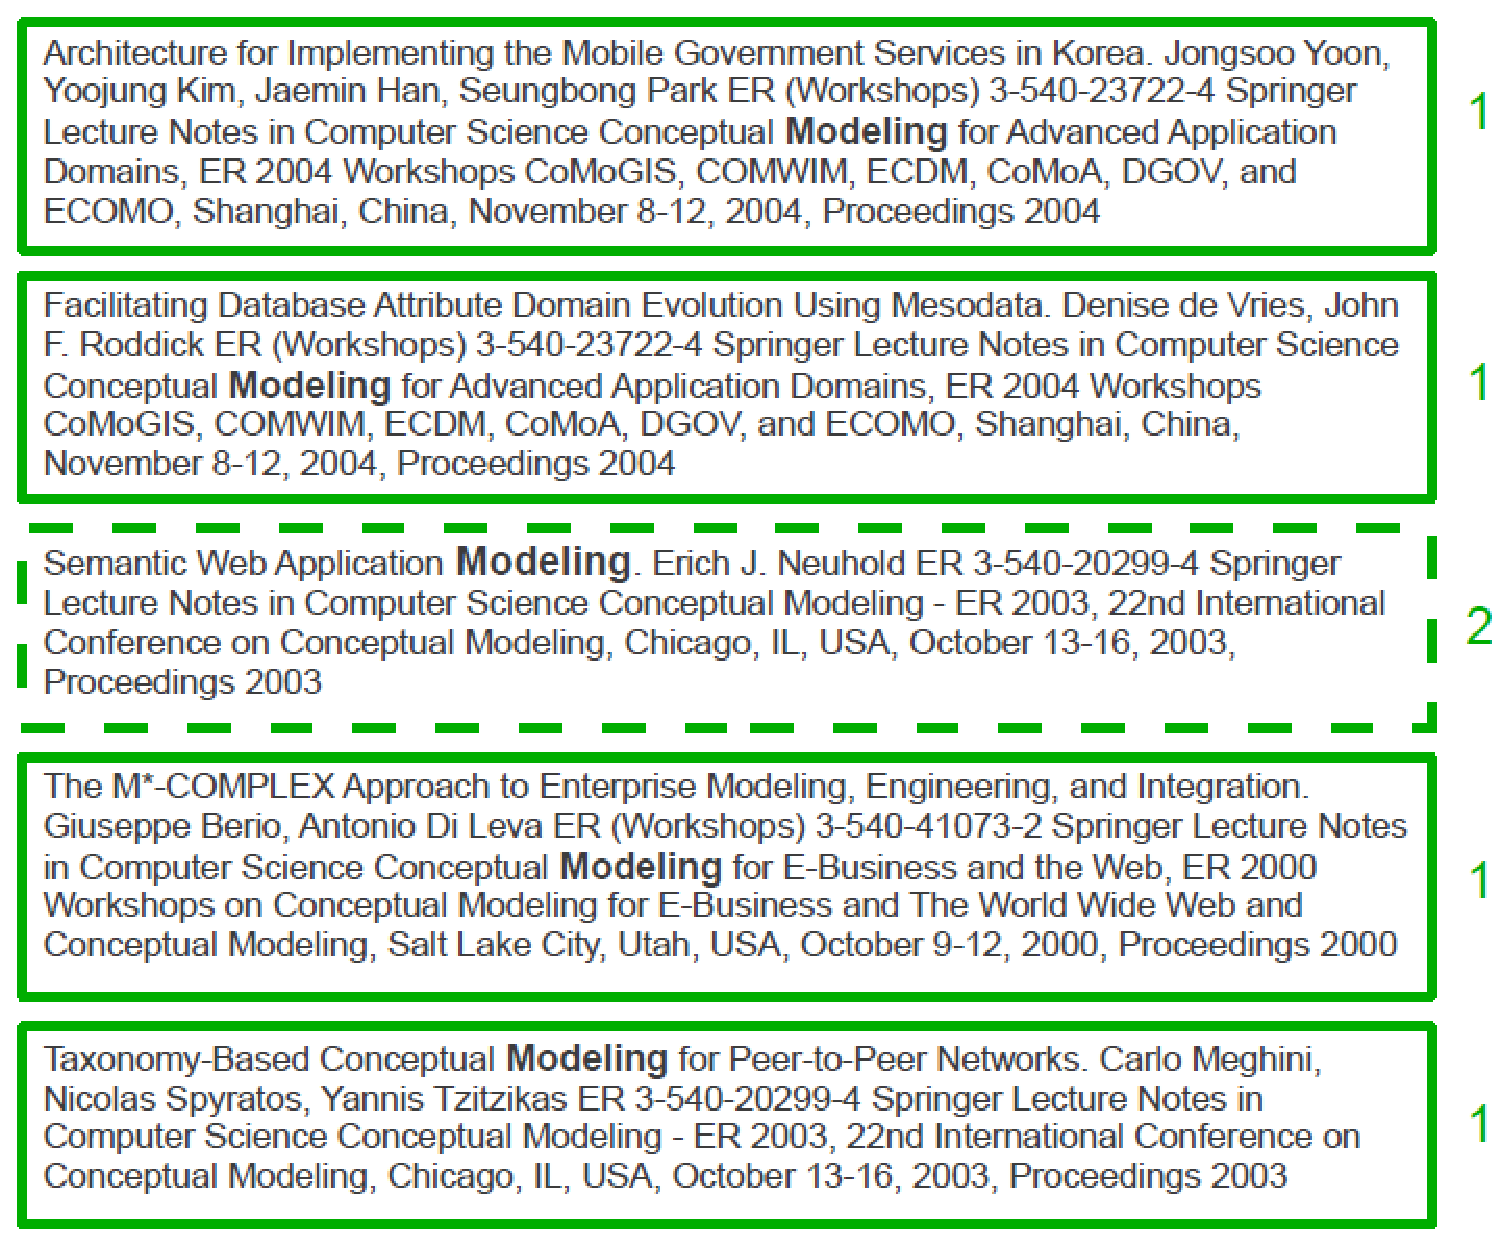
\includegraphics[width=0.47\textwidth]{cluster2.eps}
			\label{fig:token}
		}
		\subfigure[]{
			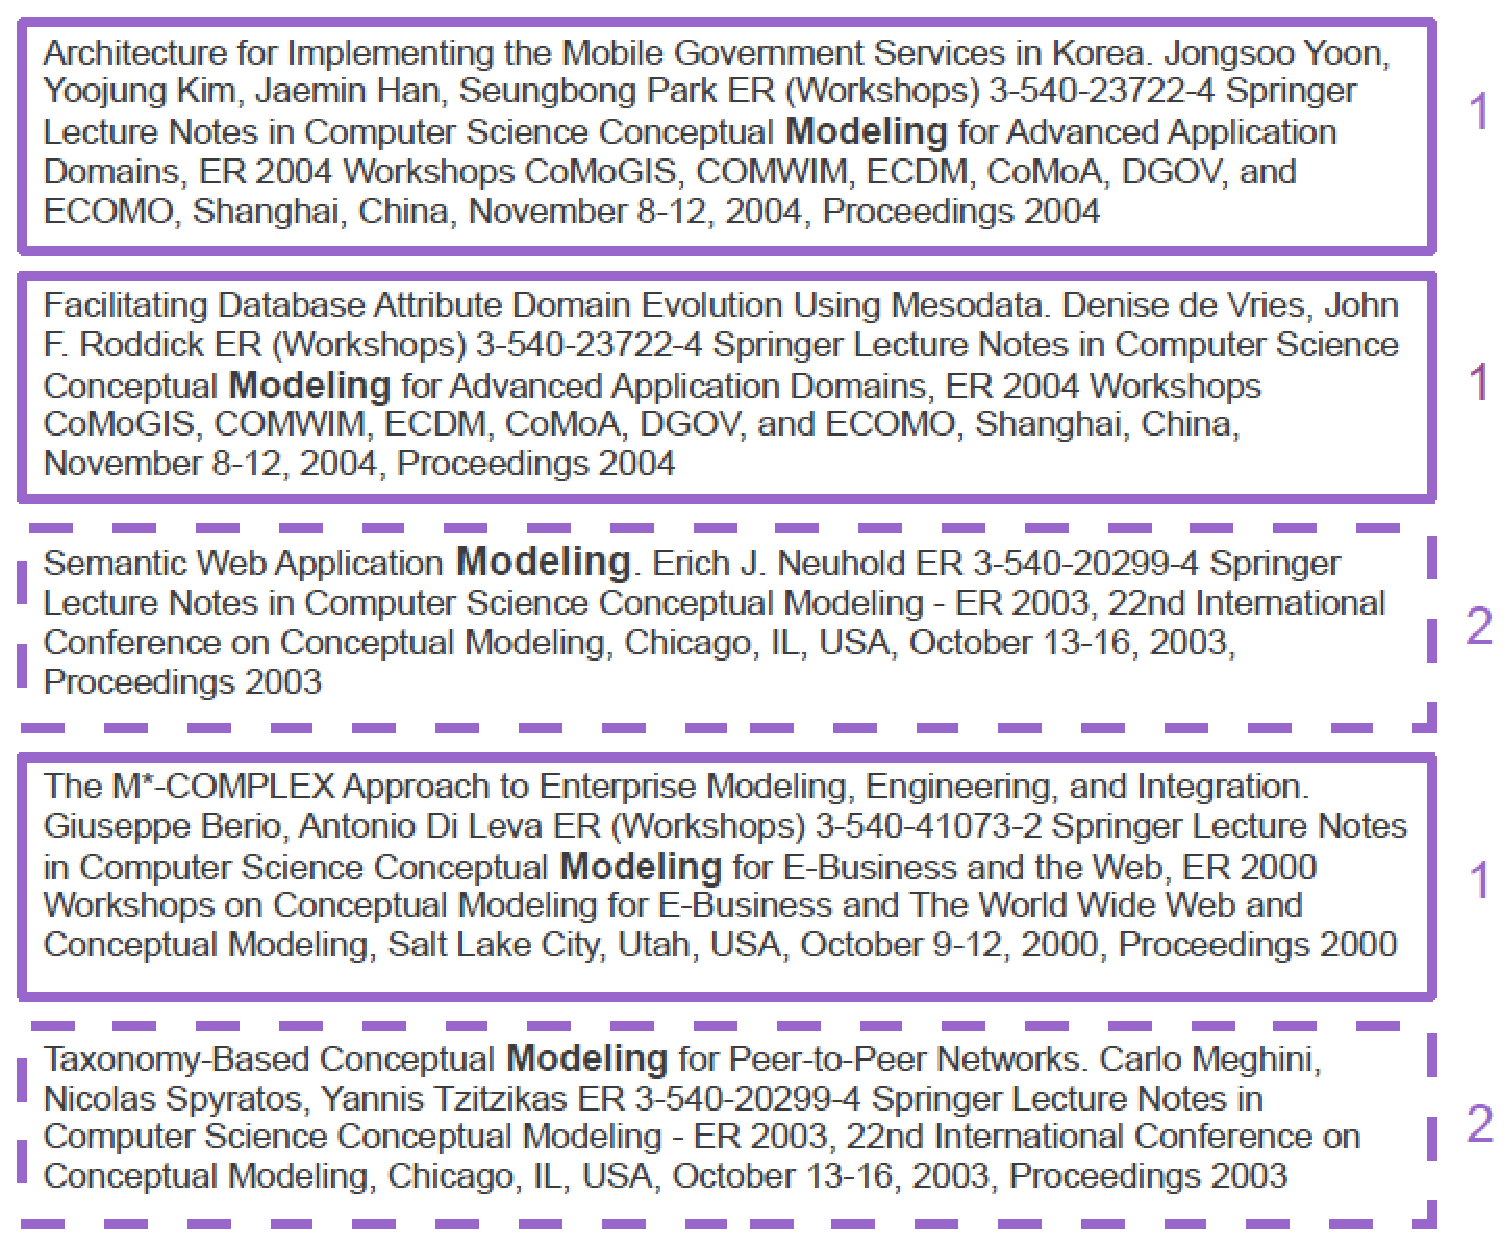
\includegraphics[width=0.47\textwidth]{cluster3.eps}
			\label{fig:label}
		}
		\caption{Clustering for the token ``Modeling'' shown over five example citations with each line type denoting a different cluster.  The level of clustering and error rate differ among whether (a) token trigrams or (b) label trigrams are used for clustering.} 
		\label{fig:cluster}
\end{figure*}

\subsection{Clustering by Information Density}

A major efficiency drawback to many active learning schemes is that they are myopic. An instance is selected
for labeling, the model is re-trained, and the process is iteratively repeated. The iterative method fails to harness the parallelizability of the crowd ecosystem. Alternativley, the faculty select tokens in batch and query the crowd at once rather than in a sequential manner. One factor that can compromise effectiveness is if there are similar token instances in the batch, as querying the label of two similar instances is equivalent to querying either of them and applying the label to both. 

We propose a scheme to cluster those tokens that should be labeled similarly and address two key issues. First, final batch must be \textit{diverse} and contain only one token from each cluster. The batch must also be \textit{dense} and contain the largest clusters whose labeling will have the greatest effect.  

In order to cluster tokens appropriately, we must define a meaningful similarity measure between them. A naive approach would cluster strictly those tokens which are equivalently out of context. This is less than desirable in our text segmentation scenario where location of the token in the document matters. Context is also important in other IE problems such as named entity recognition (NER) where homonyms with different meanings and subsequent labelings would be incorrectly grouped together.

Thus we are led to consider a \textbf{token trigram} clustering model, where tokens with similar neighbors are clustered together. Let $\mathbf{x_{i}}$ be a token at position $i$ in some document.  Together with its left and right neighbors we form the trigram $(\mathbf{x_{i-1}},\mathbf{x_{i}},\mathbf{x_{i+1}})$.  Despite being clustered as a trigram, the selection process selects the single middle token to query the crowd. We take the intuitive assumption that middle tokens $\mathbf{x_{i}}$ belonging to the same trigram are highly likely to share the same context and ought to be labeled the same. For each trigram cluster in the corpus, a single ``representative token'' with the highest mutual information (or token entropy) is selected and crowd-annotation applied to all the middle tokens in the cluster. Figure~\ref{fig:token} shows an example token trigram clustering.  

In domains such as bibliographic citation IE, many-token phrases such as common proceedings names and conference locations appear throughout multiple documents.  Common trigrams when compared across all tokens, however, are relatively infrequent. The token trigram model produces very few classification errors, but non-singleton clusters are very sparse.

There is more to the notion of context than just duplicate words appearing together. Words used in a similar ``sense" and likely to share the same label may use many different words which contextually mean the same thing. There are many ways to label how a word is used that form the fundamental backbone of NLP annotation tags, such as part-of-speech (POS), entity tags, segmentation tags, dependency parses, etc.

A token $\mathbf{x_{i}}$ has a set of associated labels $\mathbf{l_{i,j}}$, where $i$ again denotes label position and $j$ some numerical representation of the classifier type. For example, $\mathbf{l_{i,0}}$ might be the POS tag associated with $\mathbf{x_{i}}$ while $\mathbf{l}_{i,1}$ might be a segmentation tag. A \textbf{label trigram} clustering model consists of tokens that share some specified set of label trigrams. One possible cluster would be $(\mathbf{x_{i}}, (\mathbf{l_{i-1,1}},\mathbf{l_{i,1}},\mathbf{l_{i+1,1}}))$, which groups individual tokens labeled with the same segmentation tag and sharing left and right neighbors labeled the same. One requirement for all label trigram clusters is that that the individual tokens$\mathbf{x_{i}}$ should still be the same. Figure~\ref{fig:label} illustrates an example of label trigram clustering.

While these labels are themselves the uncertain output of machine learning classifers, our experiments show contextually similar tokens are also similarly mislabeled and still cluster appropriately. Overall, the label trigram model increases the recall and amount of clustering, but at the expense of a greater rate of classification error compared to the token trigram model.

Both trigram models correspond to a mapping of tokens to a lower dimensional space where tokens sharing the same trigram properties are mapped to the same point. Selecting the largest token clusters is equivalent to selecting the ``highest density" instances according to the data distribution, a technique that has shown positive yield in traditional active learning~\cite{Guo:2007:OAL:1625275.1625408}.

\eat{
\subsubsection{Clustering}
\eat{
%Individual documents, especially citation data, may contain significant overlap between authors, conferences, publishers, etc. that appear in more than one document.  While we accept a certain redundancy for quality control purposes, this should be tightly controlled through the AMT interface.  Selecting the same tokens with the same labels from different documents essentially doubles the cost for a single answer.
}

%The next optimization in the selection process is to eliminate redundant tokens in $S$. The same authors, conferences, years, etc. may be shared across multiple documents and not all tokens in $S$ may be unique.  For maximum information gain, we constrain the token set further to a set of unique tokens $R \subseteq S$.  All non-unique tokens are clustered together and single one chosen to be that cluster's \textit{representative}.  It is the representative's full document context which is sent to the crowd and the answer received is applied to all tokens in the cluster.  This allows a many-to-one relationship to exist between tokens and questions.  The choice of cluster representative is arbitrary and here we take it to be the token with the highest entropy. 

%The problem is finding such a set of representative clusters $R \subseteq S$ so that only $R$ questions need be asked to entirely cover the space of $S$.  The naive approach to clustering would be to define tokens with the same string text as being similar.  This can lead to inaccuracies for generic words.  For example, the word "computer" may appear in multiple contexts such as the title on "Human-Computer Interaction" or in a journal like "Lecture Notes in Computer Science".  See Figure~\ref{fig:cluster} for additional examples.

%We define a number of \textit{cluster properties} to ensure all tokens in a cluster should indeed be mapped to the same label.  There is a balance to be had between the size of the cluster and their accuracies.  The larger the clusters the greater impact each individual question has.  At one end of the extreme, we can group everything into one cluster so that $|R| = 1$.  Cost would be optimized, but at the expense of many mislabeled tokens.  On the other hand, everything can be grouped as a singleton so that $|R| = |S|$.  The clustering accuracy will be 100\%, but at a greater cost.  We want to define clusters in such a way that we balance between these two extremes and group tokens accurately, but not stringently, so that large clusters may develop.  In some cases, we can allow some leniency in misclustering if it's balanced out large improvement among correct clusterings.  Below we describe three sets of properties in order of decreasing selectivity of cluster admission.  The clustering process in Algorithm~\ref{alg:infoselect} is contained in lines~\ref{l:clustBegin} and~\ref{l:clustEnd} for the example set of \text{same label neighborhood} properties.


\eat{
%Our solution to this problem is through a novel clustering technique.  Tokens that share similar text and machine labeling properties have a high probability of sharing the same true labels.  By mapping multiple tokens into the same \textit{Question Cluster}, a single answer can be used to modify labels for a large number of tokens.  Whereas before we constrained the token space to the set of documents, here we constrain the space even further to only the set of unique clusters.  In the rest of this section we describe three specific cluster sets of cluster properties.

%All cluster sets require tokens belonging to the cluster to share the same token text and machine labeling, but are set apart by different neighborhood constraints.  Context is important because it's possible that two tokens with the same text such as the word "computer" could actually require different labelings and it would be false to cluster them together.  The different cluster properties trade off accuracy and cluster size and we compare them in the experiments section.  Figure~\ref{fig:cluster} compares two similar tokens and illustrates the different cluster properties that are checked.
}

%\textbf{Same Field:} The strictest of the cluster properties.  It promotes the least amount of clustering, but adheres to greatest accuracy.  The initial cluster representative defines a field by its CRF max likelihood label and all preceeding and suceeding tokens with the same label as determined by the CRF model.  Tokens are only added to the cluster if they share the entire field.  Figure~\ref{fig:field} shows an example set of five citations clustered using the Same Field method for the token \textit{Modeling}.  The first two citations share the same Proceedings field and are thus clustered together.  Whichever use of \textit{Modeling} has the highest entropy for each cluster will be that token's cluster representative.

%\textbf{Same Token Neighborhood:} The simplest of the cluster properties.  We don't check any of the machine labelings, but measure redundancy based purely on the text associated with each token.  Tokens are clustered together that share the same token as well as the same token directly preceeding and suceeding it.  This has the advantage of being purely dependent on the data and not at all on the CRF output.  This approach is slightly more error-prone.  Figure~\ref{fig:token}, which clusters by the trigram \textit{Conceptual Modeling for} shows the additional clustering that can result from this method as well as the increased possibility for error, as evinced in the final citation being incorrectly clustered with the others.

%\textbf{Same Label Neighbhorhood:} A relaxing of the Same Field properties to only compare labels one position before and after the token.  The existence of sub-entities such as a city that appears in more than one Proceedings field or an author that appears with different groups of authors motivate this approach of not checking the entire field.  Clustering is greatly increased, but at the expense of a small increase in misclassification compared to the other methods.  This is partly due to its added reliance on the machine's classification, which can contain errors.  Figure~\ref{fig:label} shows what would be expected to be a correct clustering for the token \textit{Modeling}, with cluster 1 containing those entries appearing in a Proceedings and cluster 2 those appearing in a Title.
}
\subsection{Ranking by Total Information Gain}

%Given a budget of $K < |R|$ questions, the final step is to impose a total ordering upon the set $R$ and select the top $K$.  We consider three different ways of ordering clusters for selection: by highest representative entropy, by cluster size, and by total cluster entropy.  Again, by equation~\ref{eq:condEnt}, our total utility function $H(\mathbf{Y}|\mathbf{X})$ at each step is minimized by selecting the token with the maximum marginal entropy.  We can thus order the tokens in $R$ by one at a time selecting the cluster representative with the highest entropy.  This type of ordering is ideal for applications with numerous small clusters.  For larger clusters, more information may be gained by ordering by cluster size to ensure the largest number of total tokens are covered by the budget.  For comparison, we also consider a heuristic ranking that orders by the total entropy of all tokens in a cluster, striking a balance between token marginal entropy and cluster size.  The final line of Algorithm~\ref{alg:infoselect} illustrates sorting by this metric as an example.  The various orderings are compared in our experiments in Section~\ref{sec:experiments}.

Given a limited budget of questions, clusters should be ranked to facilitate selection of the \topk.  We experimented with three different ranking schemes: ranking by mutual information score of a cluster's representative token, ranking by cluster size, and ranking by total information gain.  We define the total information gain of a cluster to be the sum of all mutual information scores of all tokens that belong to a cluster.  A comparison of the three ranking approaches can be found with the experiments in Section~\ref{sec:experiments}.
\eat{
%Adhering to our information theoretic framework, it's possible to select the "representative" high entropy token used to initiate each cluster and rank by that token's individual entropy.  On the other hand, if clusters are largely skewed in size, it may be more beneficial to rank by the actual size of the cluster.  As a final heuristic attempting to combine both the entropy and cluster size approaches, we can sort by the total entropy of each cluster, that is, the sum of entropies of every token in the cluster.  Our experiments compare and contrast these different ordering techniques.
}


\section{Uncertain Data Integration}
\label{sec:integration}

Many systems that utilize crowdsourced annotation tasks treat the results as ground truth due to the overconfidence of having a human workforce.  In practice, Turker responses have a tendency to be noisy or conflicted, thus increasing the difficulty of establishing veracity.  This means that results from the machine learning model are uncertain as well as the crowdsourced answers.  \sysName is equipped with a means of managing both types of uncertainties and integrating them into a consistent result for maximum accuracy.  In this section we motivate the need for a probabilistic approach to quality control and truth discovery and describe the generative Bayesian model implemented in \sysName.

\subsection{Probabilistic Evidence}

The de facto technique for performing quality control in a crowdsourced environment is to redundantly post the question to a number of Turkers and take a majority vote.  This naive technique is ineffective approach and there are a number reasons for wanting to pursue a probabilistic means of data integration.  

First, not all Turkers have the same capabilities and not all votes should be treated equally.  \sysName uses the expectation maximization model of Dawid \& Skene~\cite{1979} that identifies the individual reliabilities of Turkers and the confidence of their answers~\cite{Ipeirotis:2010:QMA:1837885.1837906}.  This approach has proven effective for reducing the influence of malicious workers and spammers, however, it is less suited to ambigious or difficult questions that justifiably split the workforce.  

Results are generally truncated to the maximum vote-getter and treated as truth.  Information pertaining to the ambiguity of the response is thrown out. \sysName is one of the first systems to integrate crowdsourced answers into the system in a principled manner not by replacement, but by probabilistic combination.  \sysName believes that truth should be inferred and maximum votes not taken as fact. The system treats Turker responses as individual pieces of evidence and arrives at a label distribution combining all crowdsourced information with additional information from the machine model.  

We now describe \sysName's approach in the context of the Bayesian theory of evidence.



%The current gold standard method is to ask a question to a group of people, say 3 or 5, and take a majority vote among all the answers.  While it can be an effective way of selecting the most likely answer, it is unable to handle uncertainty among the workers, which is a cornerstone of the \sysName system.  Not all Turkers have the same capabilities and not all votes should be treated equally.  In addition, even capable workers may be conflicted on difficult questions and \sysName should be able to provide a confidence level for the final aggregated response.  This allows for possible rejection of the answers or integration with machine results that have their own confidence values.

%We address these shortcomings of majority voting by developing two new \textit{uncertain integration} algorithms rooted in well known forms of probabilistic evidence management.  The first is a generative Bayesian model that establishes the CRF model as a prior and then combines crowd responses using Bayes's Rule.  The other follows the Dempster-Shafer evidence model and maps crowd and machine answers into probablistic mass functions for combination using Dempster's Rule.


\eat{
%One of the difficulties in relying on information from a crowd of sources is the possibility of a high degree of noise due to unreliable and in some cases even malicious sources.  One of the standard procedures for increasing quality control is to increase the redundancy of questions.  By asking the same question to multiple sources and aggregating the answers, we can achieve a higher probability of a good answer.

%In many cases, it suffices to collect, say, 3 or 5 votes on each question and use the majority opinion.  There are potential scenarios in which this ceases to be an effective strategy.  If the probability of receiving low quality work is equal to or greater than that of receiving higher quality, it's detrimental to treat every vote of equal merit.  Confusing or difficult questions can also cause conflict among the workers and result in a mix of answers.  Taking the deterministic mode results in a loss of information about the controversy of the question, information which may prove useful in applications such as sentiment analysis or opinion-dominated questions.

%Thus we are led to a desire to manifest the crowd response probabilistically, weighing votes proportionately and making decisions when conflicted on a question.  We implement two approaches for this data integration task, drawing separately from probability theory and belief theory.  The first maintains a single probability function, establishing a prior based on the machine's labeling, and updating the posterior using Bayes's Rule.  Alternatively, we combine the Turker response in the absence of the machine prior using Dempster-Shafer theory.  Both methods require an identification of the level of quality of each individual Turker.  We describe previous work that we've leveraged in the next section before outlining our two integration methods.\sean{Still may want to add Halpern and Fagin reference.}
}
\eat{
%\subsection{Probabilistic Integration Pipeline}

%Algorithm~\ref{alg:integration} shows the basic outline of our probabilistic integration scheme.  A first step towards probabilistic integration is to represent the data sources probabilistically, which in this case are the crowdsourced Turkers.  Each Turker is assigned a \textit{quality rating $Q$} that measures how reliable or unreliable we perceive them to be.  Explicitly, given a question, it measures the probability of the Turker choosing the correct answer versus making a random guess.  The simplest system for recovering this quality estimate, known as "honey potting", is to carefully intermix questions for which the answer is known in advance and judge Turker performance against the gold standard.  While generally effective, it lacks robustness and is defeatable to smart enough Turkers that can recognize them over time.  It is also more costly, requiring payment for answers that are already known in advance.  



%Instead, we use the expectation maximization model of Dawid \& Skene~\cite{1979} that is starting to see widespread use in crowdsourced environments~\cite{Ipeirotis:2010:QMA:1837885.1837906}.  The model requires no labeled data and alternates between choosing the correct answer from weighted Turker responses and re-evaluating those weights based on individual answers until convergence.  The final output is a set of quality ratings $Q = \{Q_{1}, \dots, Q_{m}\}$ for each worker $W = \{W_{1}, \dots, W_{m}\}$.

%Each worker provides a set of answers to K questions.  These answers $A = \{A_{1}, \dots, A_{K}\}$ along with the newly computed set of probabilities $Q = \{Q_{1}, \dots, Q_{m}\}$ for the workers are used to produce a single aggregated result using one of our two \textit{uncertain integration} methods.  The next two sections discuss the Bayesian and Dempster-Shafer models individually in greater detail.  The output using either is a single posterior probability distribution over the label space.

%In addition to \sysName aggregating answers from multiple sources, it allows the new evidence to update our initial CRF inference. Since fields are modeled with speific dependence properties, re-running the inference algorithm has the potential to change surrounding dependent fields as well.  This \textit{constrained inference} clamps the queried token to the max likelihood value and ensures all possible labelings pass through this value.  This highlights a very strong advantage of \sysName system, in that large errors can be corrected by small, incremental changes.

%The pipeline can essentially be decomposed into three distinct steps: quality estimation, answer integration, and model integration.  The first and last have appeared in previous literature.  Our main contribution is the introduction of new two methods for answer integration built from familiar probabilistic machinery.   
 }
\eat{
%Amazon Mechanical Turk provides no working system for maintaining the quality and reliability of their workforce and it is generally up to the Requester to ascertain such values on their own.    More sophisticated methods estimate quality an unsupervised manner by judging each Turker's level of agreement with the mean set of answers.  Examples include Bayesian~\cite{citeulike:9437699, DBLP:journals/jmlr/RaykarY12} methods and an approach using majority vote and expectation maximization ~\cite{Ipeirotis:2010:QMA:1837885.1837906}.

%We focus on a modified version of latter, attributable to Dawid and Skene~\cite{1979}, for implementation into \sysName .  For each question the EM algorithm takes a set of answers $a_{1}$,...,$a_{N}$ provided by N Turkers assumed to be drawn from a categorical distribution.  Associated with each Turker is a latent "confusion matrix" $\pi^{k}_{ij}$ that designates the probability the $k^{th}$ Turker will provide label $j$ when true answer is $i$.  Our modification simplifies to a binary accuracy variable $\pi^(k)$, which represents probability they will correctly label a question with the true answer.  The goal of Dawid and Skene's EM algorithm is to recover $\pi^{k}$ in the presence of the answers $a^{m}_{1}$,...,$a^{m}_{k}$ for a set of questions $m \in M$.

%In order to obtain a sufficient number of answers to similar questions by, HITs are designed in higher cost blocks.  The single task of supplying a label to a token is worth around \$0.01.  HITs are packaged in groups of 10 questions at \$0.10 each.  This ensures that if $K$ Turkers answer the HIT, relative performance can be judged across all 10 questions.

%The algorithm initializes each Turker's accuracy to 1.  It takes a majority vote among the answers to each question to define an initial answer set.  Based on this agreed upon answer set, each Turker's accuracy $\pi^{k}$ is computed.  Another majority vote weighted by $\pi^{k}$ determines a possibly different answer set.  The Turker accuracies are re-computed.  This process continues until convergence in both the "true" answer set and the $\pi^{k}$ accuracies.

%Let us take a moment to define precisely how we interpret Turker quality in the context of results of the EM algorithm.  While the Dawid \& Skene approach ultimately is calculated as correct or incorrect accuracies from a set of questions, we assume a different characteristic behavior associated with this score.  Instead of the quality being a measure of whether we believe the Turker is "correct" or not, we take quality to be a measure of \textit{reliability}.  The quality score models the probability the Turker knows the correct answer and selects accordingly, while the inverse is the probability of a \textit{random guess} from the set of possible answers.  The two approaches in the next section tackle the problem of combining responses once we have an estimate of the Turkers' quality or reliability. 
}

%~ \eat{
%~ The reason for submitting to belief theory as our main tool in the aggregation of the Turkers and machine is that it provides a natural framework arriving at a posterior distribution composed of various pieces of evidence.  While the roots of belief theory first centered around the Dempster-Shafer model, much criticism has been laid upon the model for turning up erroneous or inaccurate results.  Halpern and Fagin \cite{DBLP:journals/ai/HalpernF92} argue this is purely from a misuse of appropriating one interpretation for another.  The first view of belief function one can take is that of a generalized probability function, starting with a prior probability and updating as new evidence comes along to arrive at a conditional posterior.  On the other hand, viewing belief functions as evidence themselves leads one to use Dempster's Rule of Combination.  One presents the \textit{updating} of evidence while they other presents the \textit{combining}.  One utilizes a prior while the other does not.
%~ 
%~ We use this as inspiration for studying two different approaches to aggregating humans and machines akin to the differing interpretations.  In our Bayesian formulation, the CRF marginal distribution is used as a prior and \textit{updated} based on Turker responses.  Using an alternative Dempster-Shafer model, we forego the use of a prior and \textit{combine} Turker responses using Dempster's Rule of Combination.  
%}

\subsection{Bayesian Integration Model}

Bayesian models of evidence are initiated with some prior and updated to a posterior accounting for additional evidence. \sysName utilizes this approach by treating the machine output as the prior and human responses as the additional evidence. 

Let $A^{q} = \{A^{q}_{1}$, \dots,$A^{q}_{K}\}$ be a set of categorical random variables corresponding to the answers received from $K$ Turkers for question $q \in Q$.  The random variable $L$ follows a categorical distribution over the label space, $L_{i}$ representing the $i^{th}$ label, and $P(L)$ is the prior estimate of the label distribution for a specific token.  The choice of prior comes from the token's original CRF marginal distribution, which means we start from the machine labeling and update using new crowdsourced information.  The integration problem is to find the posterior distribution $P(L^{q}|A^{q}_{1}$,...,$A^{q}_{K})$ conditioned on the answers provided by the Turkers.  This can be calculated using Bayes's Rule:     

\begin{equation}
P(L^{q}|A^{q}_{1},...,A^{q}_{K}) = \frac{P(A^{q}_{1},...,A^{q}_{K}|L^{q})P(L^{q})}{\mathcal{Z}},
\end{equation}

where $\mathcal{Z} = \Sigma_{i}(P(A^{q}_{1},...,A^{q}_{K}|L_{i}^{q})P(L_{i}^{q}))$.  The term representing the evidence, $P(A^{q}_{1},...,A^{q}_{K}|L^{q})$, is the probability the Turker answers were generated from a specific true label.  \sysName's Bayesian model assumes Turker quality is an adequate measure of their agreement with the true label,

\begin{equation}
\label{eq:independence}
P(A^{q}_{1},...,A^{q}_{K}|L^{q}) = \prod_{k}P(A^{q}_{k}|L^{q})
\end{equation}

\begin{equation}
\label{eq:bayes_evidence}
%P(A^{n}_{k}=a|L^{n}=l) = |\mathbbm{1}_{{a}\neq l} - Q_{k}| + |\mathbbm{1}_{a=l}-Q_{k}|*\frac{1}{|L|}
P(A^{q}_{k}=a|L^{q}=l) = 1{\hskip -2.5 pt}\hbox{I}_{{a}= l}* Q_{k} + (1-Q_{k})*\frac{1}{|L|}
\end{equation}

where $a$ and $l$ are values drawn from the label space and $Q_{k}$ is the quality of the k$^{th}$ worker.  Equation~\ref{eq:independence} follows from all Turker answers being independent of each other and equation~\ref{eq:bayes_evidence} simply restates our assumption about the use of Turkery quality $Q_{k}$.  If the answer matches the label $l$, the first term on the right hand side is the probability the Turker is reliable and answers the question truthfully.  The second term incorporates the probability they are unreliable or a spammer and through \textit{random guessing} finds the correct answer with probability $1/|L|$, $|L|$ being the number of possible labels.  If they don't match, we have the probability the Turker is unreliable, $1-Q$, and the probability a random guess produces an incorrect answer, $(L-1)/L$.
 
The full model to obtain the probability of a label $L^q$ given turker answers $A^{q}_1 \ldots A^{q}_K$ is

\begin{align}
\label{eq:full_bayes}
P(L^{q}&=l|A^{q}_{1}=a_{1},...,A^{q}_{K}=a_{k}) = \nonumber\\
                 &\frac{1}{Z}P(L^{q}=l)\prod_{k}\big(1{\hskip -2.5 pt}\hbox{I}_{{a_{k}}=l} *Q_{k}  + (1-Q_{k})*\frac{1}{|L|}\big)
%P(&L^{n}=l|A^{n}_{1}=a_{1},...,A^{n}_{K}=a_{k}) = \\
%&P(L^{n}=l)\prod_{k}\big(|\mathbbm{1}_{{a_{k}}\neq l} - Q_{k}|  + |\mathbbm{1}_{a_{k}=l}-Q_{k}|*\frac{1}{|L|}\big)
\end{align}

Using equation~\ref{eq:full_bayes} for all possible labels $l$ and renormalizing produces a new posterior distribution accounting for both the initial ML extracted result and evidence gathered from the crowd.  The product can even be extended and updated as new evidence comes in over time allowing for a persistently updateable system of truth management.  This approach has been considered using a different technique in~\cite{Sheng:2008:GLI:1401890.1401965}.  While currently evidence is designed to come from the crowd in \sysName , there is no explicit restriction preventing future updates from incorporating evidence from a number of different extractions as well as the crowd.  We close this section with an example to better illustrate the integration algorithm.

\begin{example}
\label{ex:bayes}
Assume a binary question is answered by three Turkers.  Turker A has quality 0.9 and answers with label 0, Turker B has quality 0.4 and answers with label 1, and Turker C also has quality 0.5 and also responds with label 1.  The prior CRF marginal probability over \{0,1\} is \{0.5,0.5\}.  A majority vote among the three Turkers would give label 1, even though both are of relatively low quality.  The Bayesian combination can be found from equation~\ref{eq:full_bayes}, 
%\begin{equation}
\begin{align}
P(L=0|&A,B,C) \nonumber\\
&= P(L=0)P(L=0|A)P(L=0|B)P(L=0|C)\nonumber\\
	        &= (0.5)\left(0.9 + (0.1)(\frac{1}{2})\right)(0.6)(\frac{1}{2})(0.5)(\frac{1}{2})\nonumber\\
	        &\approx .036\\
P(L=1|&A,B,C) \nonumber\\
&= P(L=1)P(L=1|A)P(L=1|B)P(L=1|C)\nonumber\\
	        &= (0.5)(0.1)(\frac{1}{2})\left(0.4 + (0.6)(\frac{1}{2})\right)\left(0.5 + (0.5)(\frac{1}{2}\right)\nonumber\\
	        &\approx .013
\end{align}
%\end{equation}
After combining and normalizing, the final distribution over \{0,1\} is \{0.73,0.27\}.  Instead of truncating and taking label 0 as truth, this binary distribution would be retained in the system.  If task the budget were to increase, this question might be chosen again and the distribution refined even further.
\end{example}

\subsection{Data Integration Pipeline}

Here we briefly summarize for clarity the entire data integration pipeline in Algorithm~\ref{alg:integration}.  After questions have been selected based on the techniques described in Section~\ref{sec:selection}, the HIT Management module produces questions and posts them to Amazon Mechanical Turk, the results of which are automatically retrieved and stored in the database.

Questions are posted as HITs in batches of size N.  The fixed batch size ensures that enough Turkers answer the same questions for the EM process.  For a set of M Turkers answering an HIT of N questions, we use Dawid \& Skene to estimate accuracies for each Turker.  These accuracies are saved in a table in the database so if a worker performs more than one HIT their accuracies for each one are averaged together.  Recording the history of turker accuracy is an additional benefit of having a persistent system.

For each question, the Turker accuracies and answers are integrated with model output using the Bayesian framework described in the previous section.  This produces a distribution over the label space.  Since queried tokens were pulled from clusters as per Section~\ref{sec:selection}, the answer corresponds to the selected ``representative token".  The entire reason for clustering, however, was to map this distribution back to all the tokens belonging to the same cluster and satisfying some similarity threshold.  Therefore, all token accuracies belonging to a selected cluster get updated.

For all documents containing tokens that were updated, constrained Viterbi inference is performed, the constraint being that the incoming transition probability is reflective of the new updated marginal distribution.  The final labeling represents an efficient integration of both human and machine computation. 

\begin{algorithm}[fillcomment]
\label{alg:integration}
\SetKwInOut{Input}{input}\SetKwInOut{Output}{output}
\Input{Set of clusters $C$,\\
CRF prior for each cluster\\}
\Output{Labeled document d\_labeled}
\BlankLine
\CommentSty{//Query AMT for responses}\;
\lnl{}ans $\leftarrow$ queryAMT()\;
\CommentSty{//Calculate Turker qualities}\;
\lnl{}qual $\leftarrow$ Dawid\_Skene(ans)\;
\CommentSty{//Compute posterior distribution of answers}\;
\lnl{}combo\_ans $\leftarrow$ Bayesian\_integrate(pr, ans, qual)\;
\CommentSty{//constrain CRF for all tokens in clusters}\;
\ForEach{cluster $c$ $\in$ C}
{
    \ForEach{tok $\in$ cluster $c$}
        {
            \lnl{}(docID, pos) $\leftarrow$ getToken(tok)\;
            \lnl{}CRF(docID,pos) $\leftarrow$ combo\_ans(c)\;
	 \lnl{}RunViterbi(CRF(docID,pos))\;
        }  
}
\caption{Probabilistic Integration}
\end{algorithm}

\eat{
\subsection{Dempster-Shafer Integration Model}
%~ \eat{
%~ A viable alternative is to exhibit no faith in the machine's initial marginal calculation.  After all, one could argue that by selecting only the most uncertain tokens that metric loses its value.  
%~ }

%In contrast to the Bayesian evidential model of updating a prior, the Dempster-Shafer model~\cite{shafer1976mathematical} makes no such assumption that a prior exists or is useful.  It instead seeks to combine multiple disparate forms of evidence, which are represented as mass or belief functions.  While probability theory ascribes the likelihood of single events, belief theory assigns mass to \textit{sets} of outcomes.  For example, in the flipping of a coin, a probability can only be assigned to $H$ (heads) or $T$ (tails), while belief can additionally be defined over the ambiguous set $\{H,T\}$ representing \textit{either} outcome.  Belief functions do not necessarily have to add up to $1$, though we retain this principle for simplicity without loss of generality.

\eat{
%While the Bayesian approach was inspired by an alternative interpretation of belief functions, the actual implementation is still a probability function through and through, with all of Kolmogorov's axioms defining a probability function still holding.  For evidential combination, however, we leverage the full power of belief theory and relax some of those axioms to map to a set of belief functions.  

%The main difference between a belief function and a probability function is that probability functions are defined only over the \textit{measurable} subsets of a set while belief functions are defined over \textit{all} subsets (the power set) of a set~\cite{shafer1976mathematical}.
}
\begin{example}
\label{eq:coin1}
We can assign simple belief functions to the flipping of a coin as per our earlier example.
\begin{align*}
m({H}) &= 0.4\\
m({T}) &= 0.2\\
m({H,T}) &= 0.4
\end{align*}
%The intuitive understanding of the above assignments is that we are 40\% certain that the outcome will be heads, 20\% certain that the outcome will be tails, and 40\% certain that the outcome will be either heads or tails, which is equivalent to being 40\% uncertain of the outcome (clearly we don't expect this to be a fair coin).  This formalism provides a natural bookkeeping for uncertainty management.
\end{example}
%Belief functions are important representations of evidence because they can be integrated using Dempster's Rule of Combination to reach a consensus.  The coin example above might represent one source's expectation of the coin's probabilities.  If another source weighed in with a different set of expectations, the two may be combined into a single model of the coin's fairness (or lack thereof).  No additions are made to the core of the Dempster-Shafer evidence model.  Our contribution lies in a unique way of assigning Turker answers to belief functions which reinforces our notion of Turker reliability.

%Like with the Bayesian approach, our confidence in the correct answer is reflected in their Quality score.  Let $\mathcal{A}$ be the set of all possible labels ${1,2,...,L}$, akin to ${H,T}$ from Example~\ref{eq:coin1}.  We assume in this framework that Turkers are either reliable, getting the answer correct with belief score $Q_{k}$, or unreliable, reflected in a random guess with belief score $1-Q_{k}$.  While the use of mass functions has a long history, this assignment to reflect source accuracy is unique to the best of our knowledge.  Explicitly, for a Turker $k$ with provided answer of $a_{k}$ to the $n^{th}$ question:

\begin{equation}
m^{n}(\{2^{L}\}) = 0
\end{equation}
\begin{equation}
\label{eq:mass1}
m^{n}(\{a_{k}\}) = Q_{k}
\end{equation}
\begin{equation}
\label{eq:mass2}
m^{n}(\mathcal{A}=\{1,\dots,L\}) = 1-Q_{k}
\end{equation}

%The first equation simply states that we initialize all mass functions to zero before setting the two values below it.  After initialization, the mass corresponding to the Turker's response is set to the quality value $Q_{k}$ while the mass of the set containing all labels consists of the remaining probabilistic mass.  Thus equation~\ref{eq:mass1} reflects how certain we are in the answer and equation~\ref{eq:mass2} shows how uncertain.  Clearly a reliable Turker will have more mass peaked in the region of certainty than an unreliable one.  The set of mass functions from multiple Turkers can be combined using Dempster's Rule of Combination, which combines mass functions in a pairwise manner:

\begin{equation}
\begin{split}
\label{eq:DS_combo}
m_{1,2}(A) &=(m_{1}\oplus m_{2})(A)\\
                   &=\frac{1}{1-K} \sum_{B\cap C=A\neq\emptyset} m_{1}(B)m_{2}(C),
\end{split}
\end{equation}

\begin{equation}
\label{eq:K}
K=\sum_{B\bigcap C=\emptyset}m_{1}(B)m_{2}(C).
\end{equation}

%Dempster's Rule is essentially an outer product over all sets that share a common intersection, normalized by a factor that includes the number of mutually exclusive sets.  The combination is both associative and commutative.

%Our application of the procedure is to map all HIT responses to mass functions and combine them one-by-one in turn to produce a single combined mass function $m_{comb}$.  Any remaining uncertainty in $m_{comb}(\mathcal{A})$ is added to all the singleton functions and re-normalized to produce a single probability function.  The original belief formulation is also stored in \sysName in case new evidence arrives at a later time.

\begin{example}
\label{ex:DS}
Given the same Turkers and answers from Example~\ref{ex:bayes}, Dempster's Rule of Combination may also be used to combine them.  First, we map them to mass functions using equations~\ref{eq:mass1} and ~\ref{eq:mass2}:
\begin{align*}
m_{A}(\{0\}) = 0.9, \text{ } m_{A}(\{1\}) &= 0, \text{ } m_{A}(\{0,1\}) = 0.1\nonumber\\
m_{B}(\{0\}) = 0, \text{ } m_{B}(\{1\}) &= 0.4, \text{ } m_{B}(\{0,1\}) = 0.6\nonumber\\
m_{C}(\{0\}) = 0, \text{ } m_{C}(\{1\}) &= 0.5, \text{ } m_{C}(\{0,1\}) = 0.5
\end{align*}
We apply equations~\ref{eq:DS_combo} and~\ref{eq:K} to combine Turkers A and B, and then the result is combined with Turker C.  We leave off the K term as it applies to all of the following equations and does not change the relative distribution.
\begin{align*}
m_{A,B}(\{0\}) &= m_{A}(\{0\})m_{B}(\{0,1\}) = 0.54\nonumber\\
m_{A,B}(\{1\}) &= m_{B}(\{1\})m_{A}(\{0,1\}) = 0.04\nonumber\\
m_{A,B}(\{0,1\}) &= m_{A}(\{0,1\})m_{B}(\{0,1\}) = 0.06\nonumber\\
\vspace{2mm}
m_{A,B,C}(\{0\}) &= m_{A,B}(\{0\})m_{C}(\{0,1\}) = 0.27\nonumber\\
m_{A,B,C}(\{1\}) &= ((m_{A,B}(\{1\})m_{C}(\{1\})\nonumber\\
	 &+ m_{A,B}(\{0,1\})m_{C}(\{1\})\nonumber\\
	 &+ m_{A,B}(\{1\})m_{C}(\{0,1\})) = 0.07\nonumber\\
m_{A,B,C}(\{0,1\}) &= m_{A,B}(\{0,1\})m_{C}(\{0,1\}) = 0.03
\end{align*}
%To convert to a probability distribution, we add $m_{A,B}(0,1)$ to each of the individual components and normalize.  The final distribution over \{0,1\} is \{0.75,0.25\}, nearly identical to the result of Example~\ref{ex:bayes}.
\end{example}

%While we introduce Dempster-Shafer theory here in the context of our simpler one-answer-per-question framework currently found in \sysName , it is not to be taken in contrast with its Bayesian counterpart, but as a generalization of it.  The method will become more powerful in future work where we plan to extend functionality to allow the Turkers to provide more than one response per question when uncertain.  Reasoning over such fuzzy sets exemplifies the real power for using belief theory over probability theory.
}
\eat{
\subsection{Quantifying Turker Performance}

The previous section looked at ways to combine Turker answers probabilistically to arrive at a final result that is not deterministic.  This is useful for when there is controversy or confusion elicited over the answers of a question.  We use the entropy of the final label distribution to arrive at confidence value for each question.  Depending on the required accuracy of the application, a threshold on the confidence may be placed to assure only the highest quality results make it through.  In the experiments we highlight Receiver Operating Characteristic (ROC) curves that measure performance vs. answer recall.  Answers not making the cut may have their questions re-submitted to attain more information in discerning the result. 
}



\section{Experiments}
\label{sec:experiments}

\begin{figure*}[t]
    \centering
    \subfigure[] {
        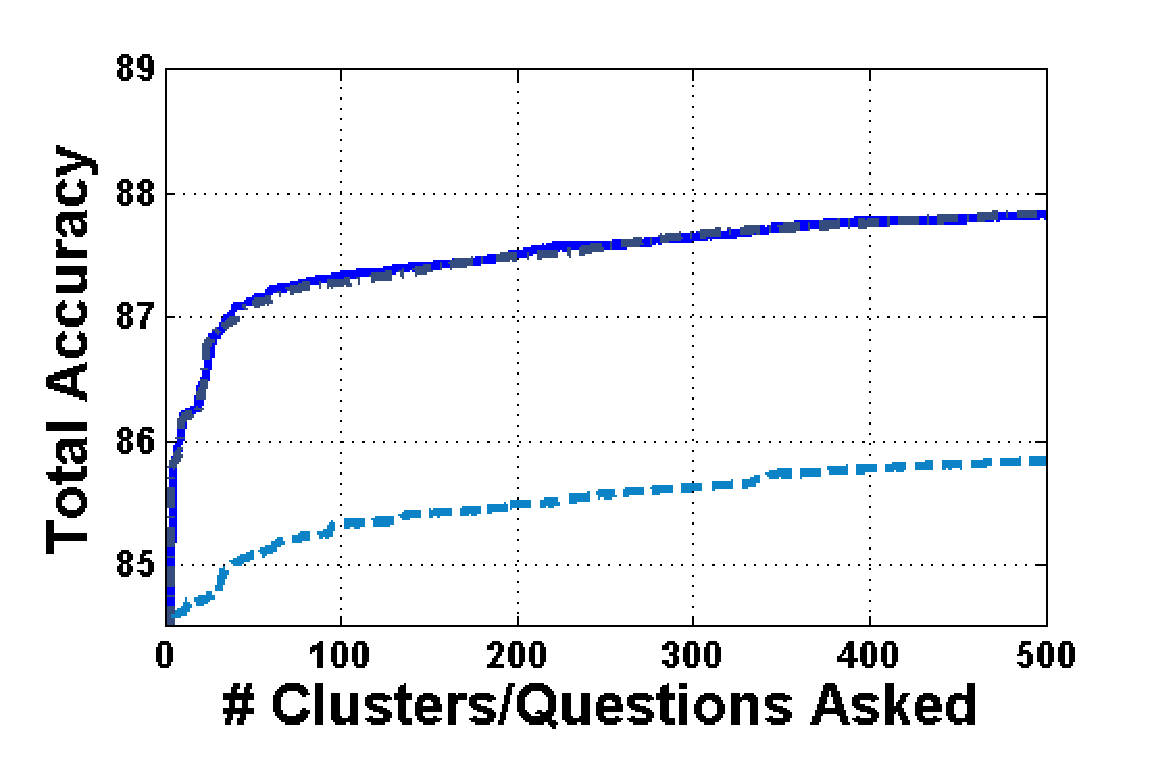
\includegraphics[width=0.31\textwidth]{dblp_seeding_compare.eps}
        \label{fig:first1}
    }
    \subfigure[] {
        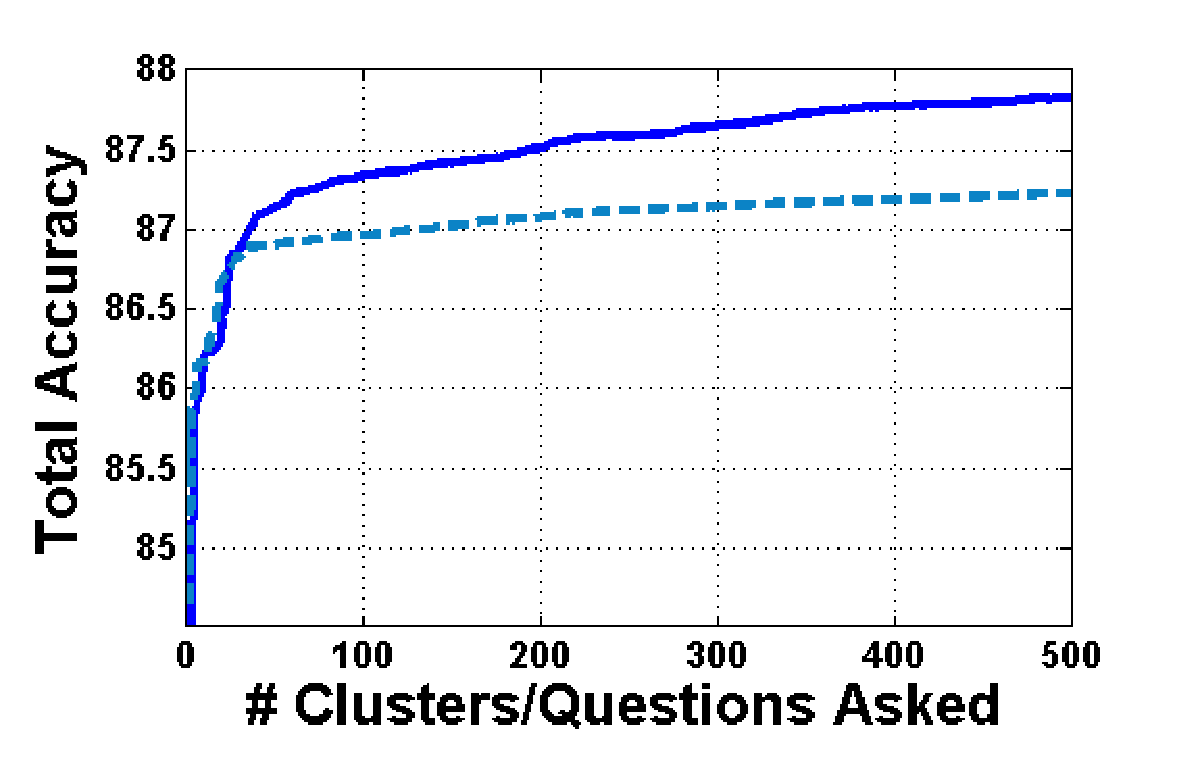
\includegraphics[width=0.31\textwidth]{dblp_clustering_compare.eps}
        \label{fig:first2}
    }
    \subfigure[] {
        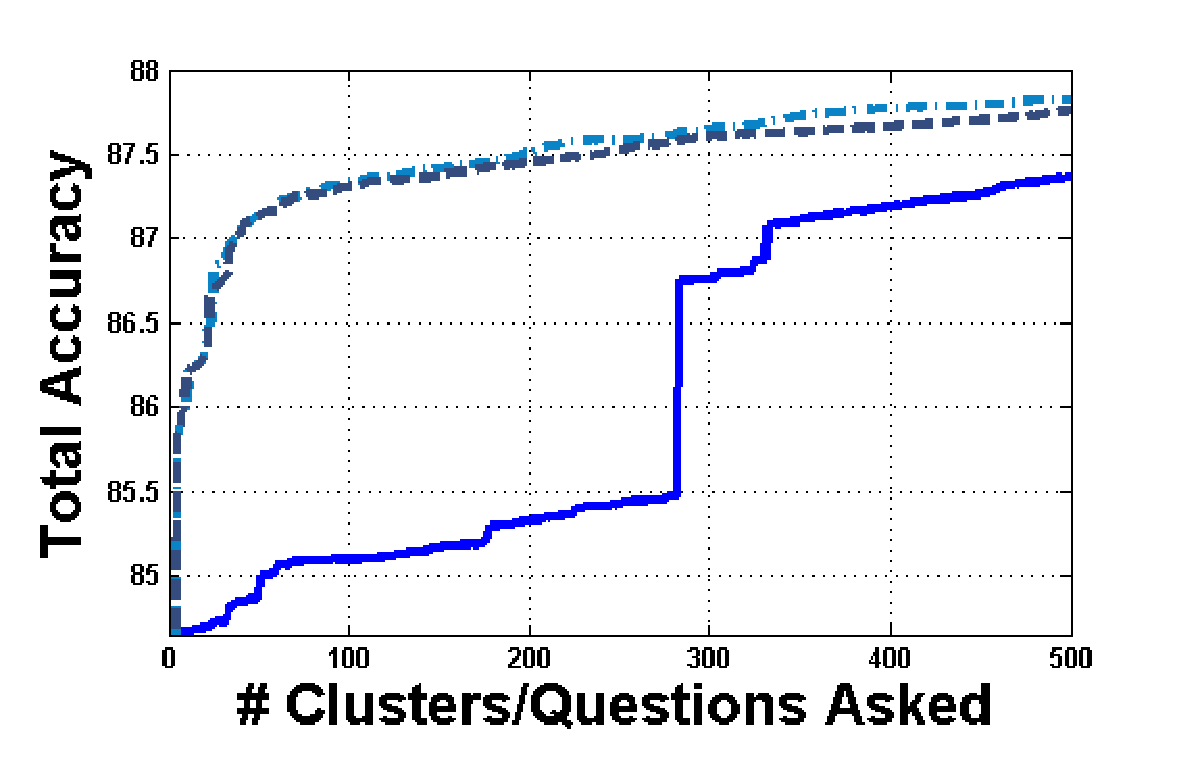
\includegraphics[width=0.31\textwidth]{dblp_ranking_compare.eps}
        \label{fig:first3}
    } \\
    \subfigure[] {
        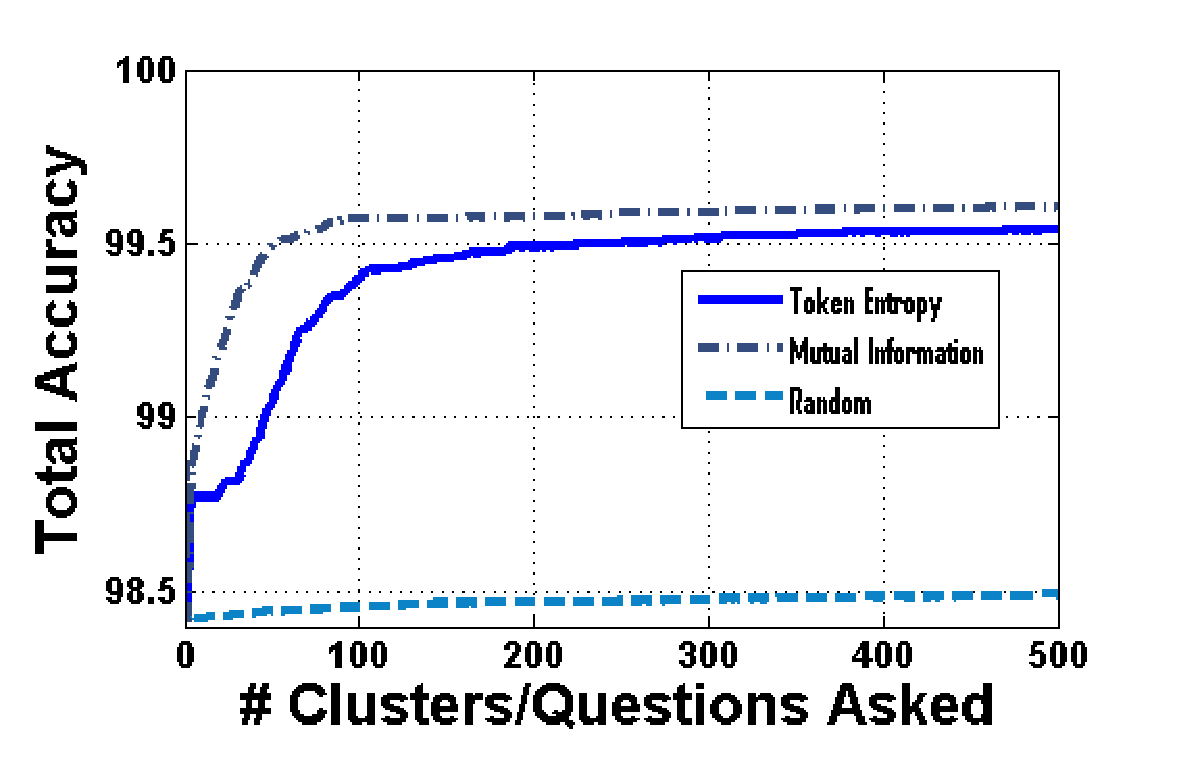
\includegraphics[width=0.31\textwidth]{pubmed_seeding_compare2.eps}
        \label{fig:first4}
    }
    \subfigure[] {
        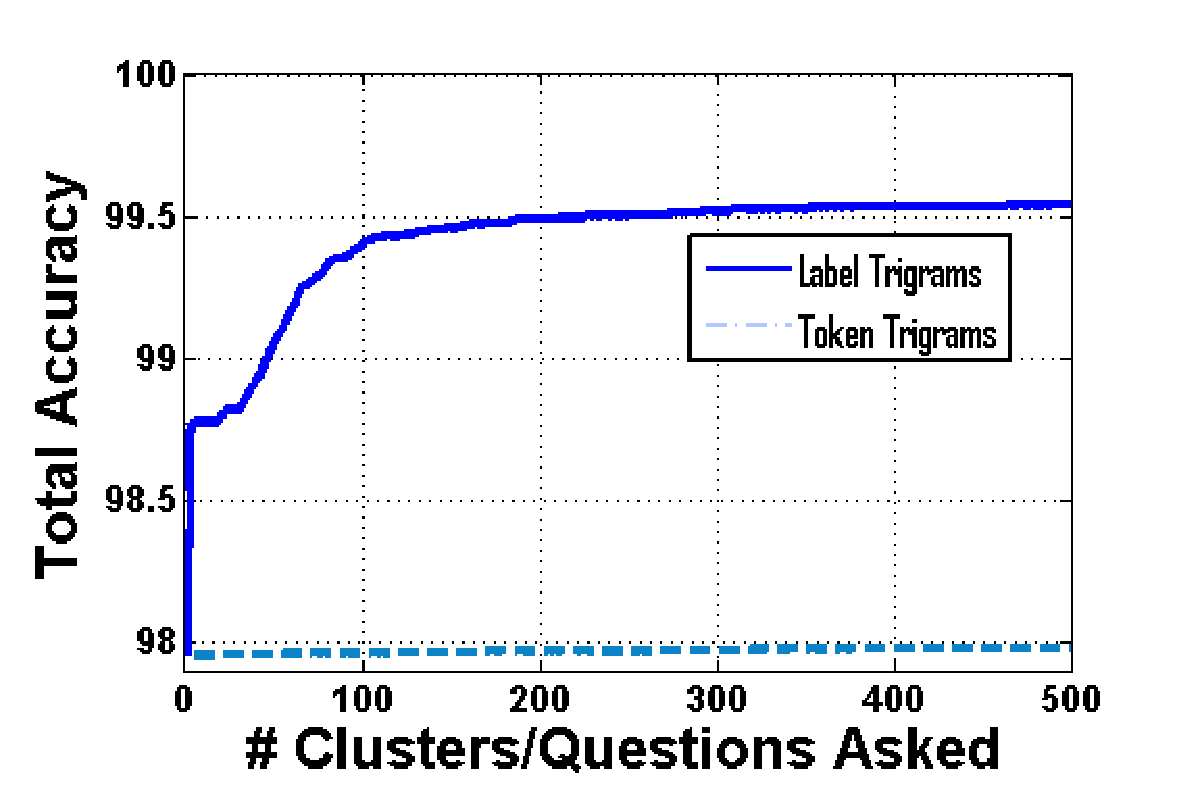
\includegraphics[width=0.31\textwidth]{pubmed_clustering_compare2.eps}
        \label{fig:first5}
    }
    \subfigure[] {
        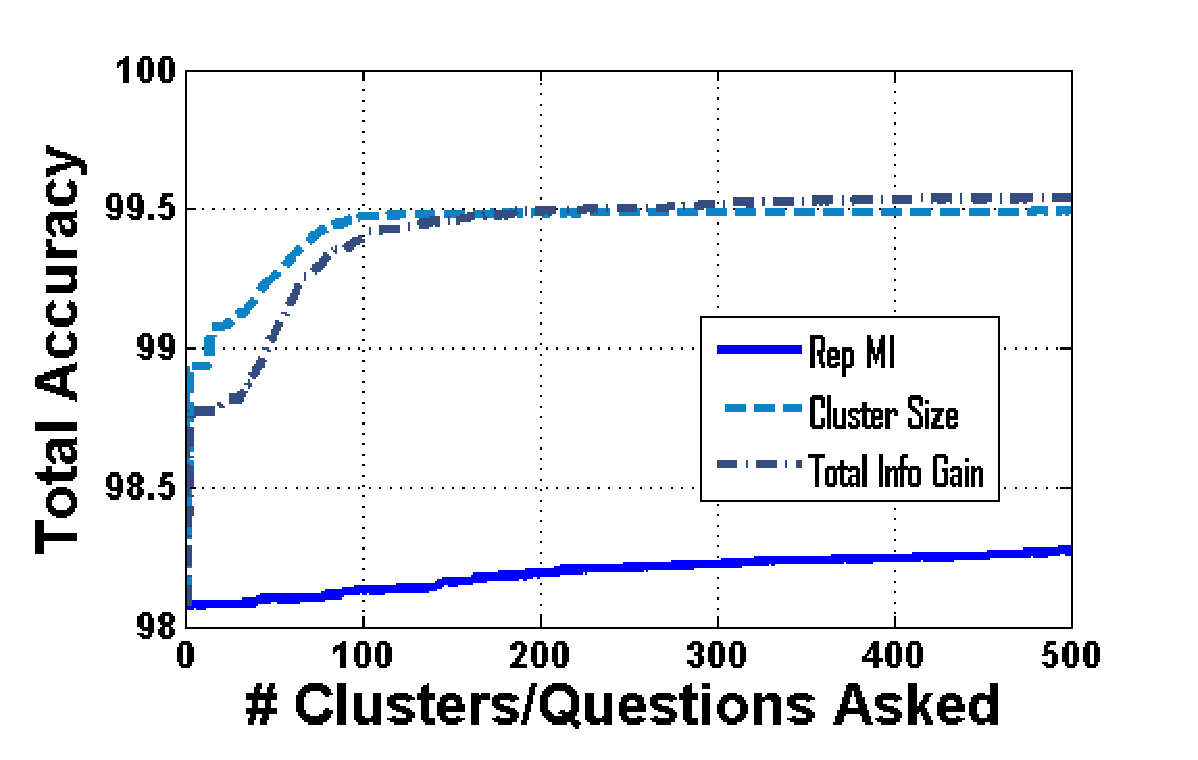
\includegraphics[width=0.31\textwidth]{pubmed_ranking_compare2.eps}
        \label{fig:first6}
    }
    \caption{Accuracy improvements for various selection parameters.  The first row is for the DBLP data set and the second is for PubMed.  From the left to right the columns compare the filtering, clustering, and ranking methods mentioned in this paper.  The parameter legend applies to both plots in each column.  Where not explicily being compared, the defaults are Mutual Information, Same Label, and Total Information Gain, respectively.}
    \label{fig:selectionExp}
\end{figure*}

In this section we demonstrate the effectiveness of our selection and integration approaches on sets of synthetic and real data.  

\subsection{Setup and Data Sets}
\label{sec:setup}

We extracted 14,000 labeled citations from the DBLP\footnotemark\footnotetext[1]{http://kdl.cs.umass.edu/data/dblp/dblp-info.html} and 500,000 from the PubMed\footnotemark\footnotetext[2]{http://www.nlm.nih.gov/bsd/licensee/medpmmenu.html} databases.  For unlabeled testing data, we removed the labels and concatenated text from each of the available fields.  Order of fields was randomly mixed in keeping with real-life inconsistency of citation structure.

To test our selection methods without the effects of integration accuracy, we supplemented the ground truth values in place of Turker answers when running constrained inference, equivalent to a workforce of perfect Turkers.  To evaluate the integration techniques, we experimented with simulated answers as well as real answers from AMT.  For answer simulation we sampled the accuracy $Q_{i}$ of Turker $i$ from a normal distribution $\mathcal{N}(\mu,~\sigma)$ whose parameters we allowed to vary.  Where not listed explicitly, we used the values $\mu=0.5$ and $\sigma=0.3$.  We sampled the ground truth value with probability $Q_{i}$ and with probability $1-Q_{i}$ a random guess was used instead.

We also performed a set of experiments on Amazon Mechanical Turk using both datasets while varying question difficulty.  Each HIT consisted of 10 bibliographic token annotation tasks at \$0.10 per HIT, or \$0.01 per token. From the DBLP set we produced a set of 500 HITs and required users to pass a qualification test before being allowed to answer questions.  We produced an additional ``hard" set where the same questions were stripped of any punctuation and no qualification test was used.  The motivation was to develop questions of a more ambiguous nature likely to cause more conflicts.  We coined this set DBLP-hard.  The PubMed set consisted of 500 questions and also required no such qualification test.  Some of the more ambiguous questions were selected to further test confusion among Turkers and study conflict.  In all sets 5 Turkers were assigned to each HIT and quality was assessed on a per HIT basis using the Dawid \& Skene method.

\subsection{Selection Experiments}

%\begin{figure}
    %\centering
    %\subfigure[DBLP] {
        %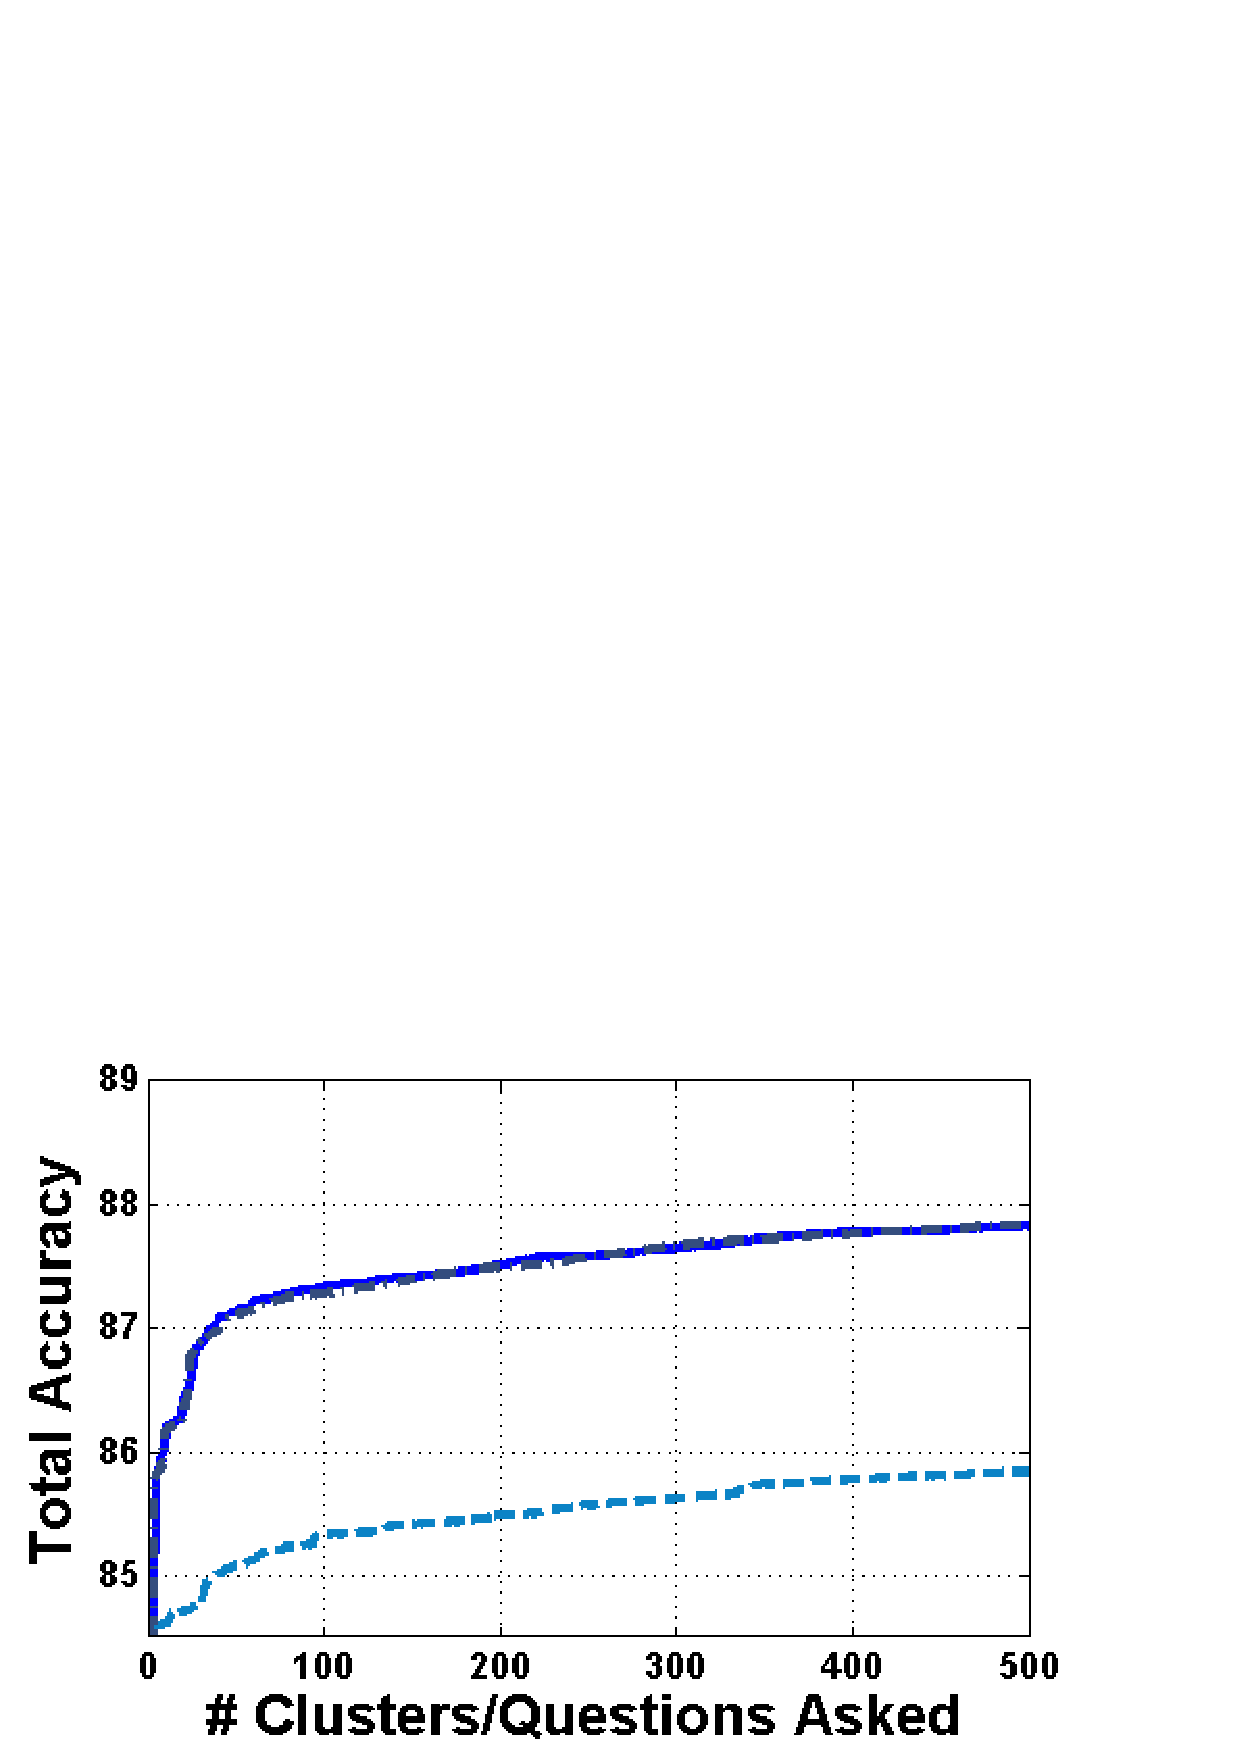
\includegraphics[width=0.22\textwidth]{images/dblp_seeding_compare.png}
        %\label{fig:first1}
    %}
    %\subfigure[PubMed] {
        %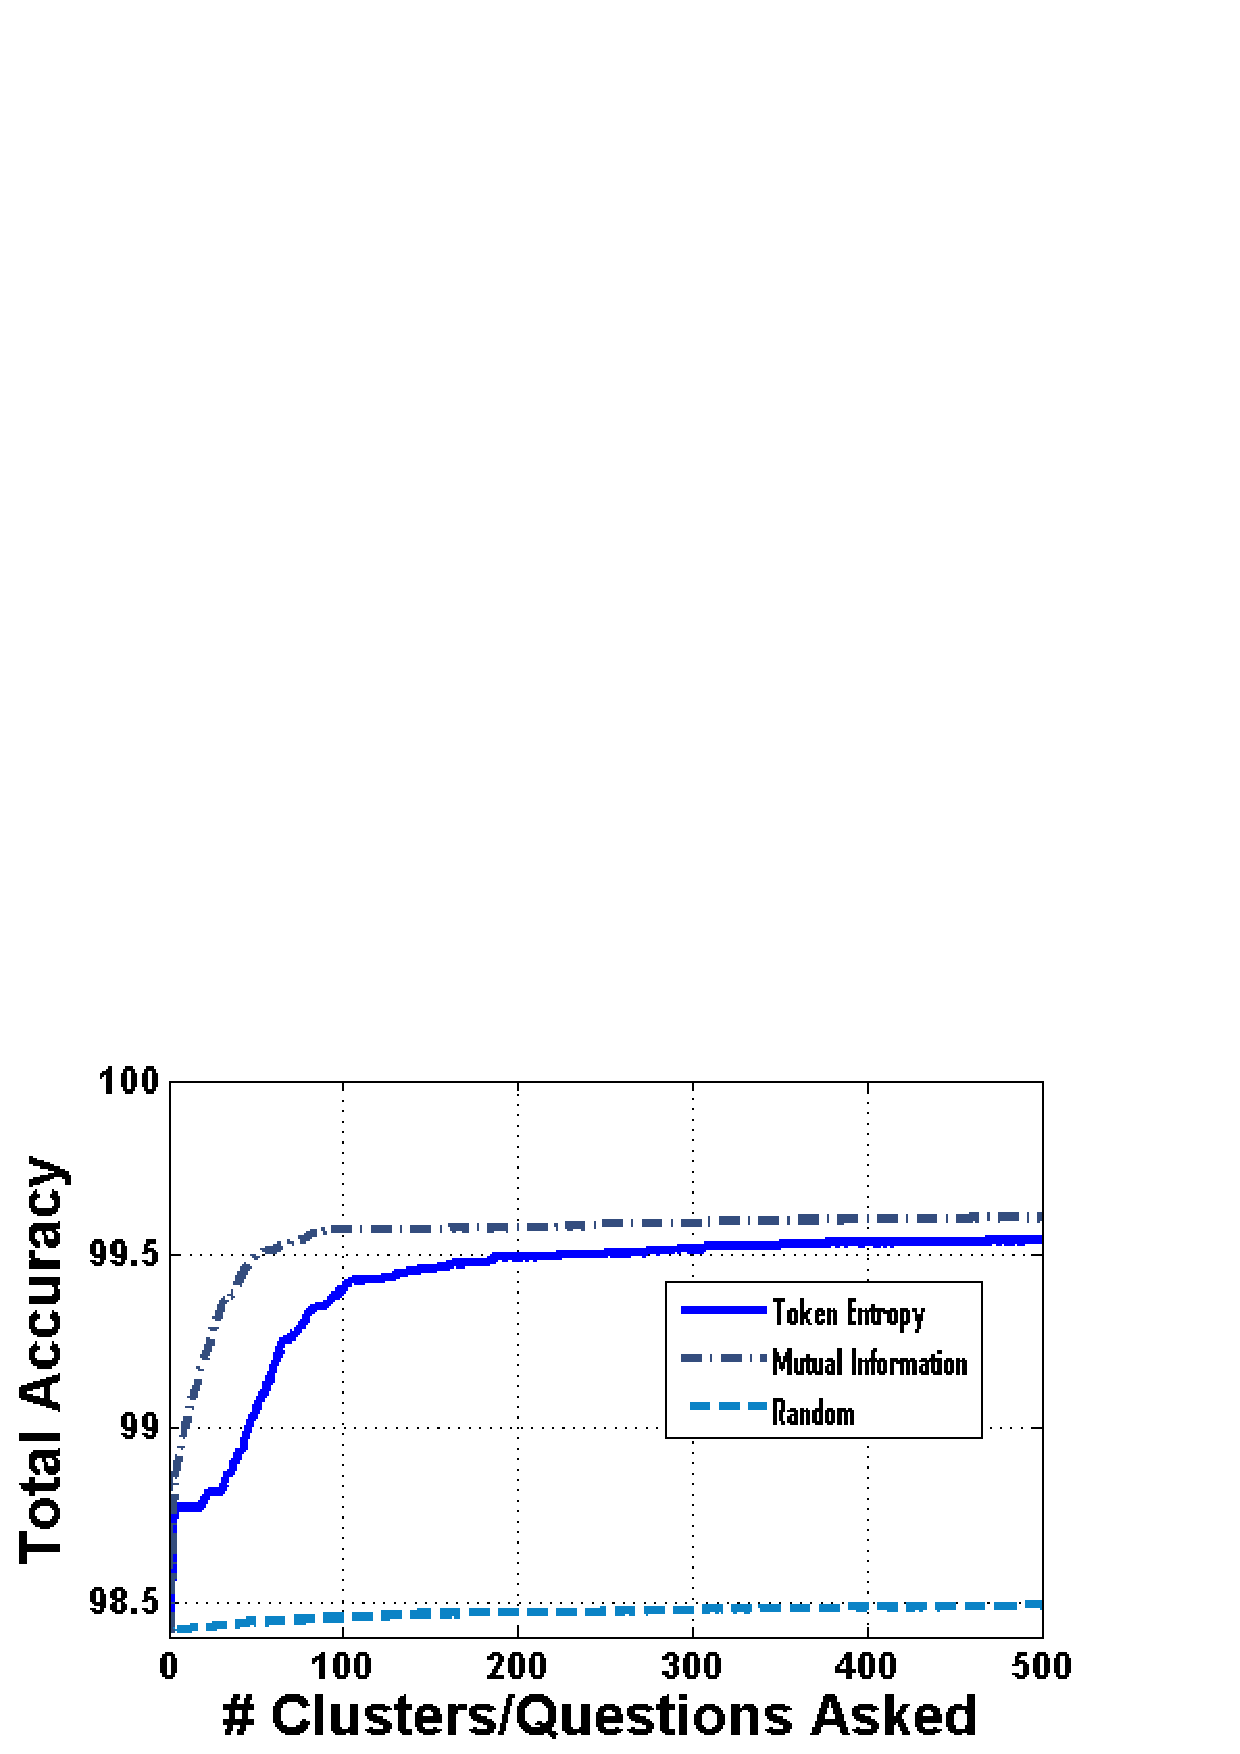
\includegraphics[width=0.22\textwidth]{images/pubmed_seeding_compare2.png}
        %\label{fig:second1}
    %}
    %\caption{Seeding comparison for (a) DBLP and (b) PubMed.  Default clustering is Same Label and default ranking is Total Entropy.}
    %\label{fig:select1}
%\end{figure}

Figures~\ref{fig:first1}-\ref{fig:first6} contain experiments comparing our various selection algorithms by detailing the accuracy improvements after a specific number of questions have been asked.  Tokens were selected based on the pipeline of Algorithm~\ref{alg:QuestionSelect} using a specific combination of filtering, clustering, and ranking approaches.  The choices for filtering were random selection, highest token entropy, and highest mutual information.  Clustering compares the token trigram and label trigram methods.  Finally, ranking looks at ordering by highest representative token mutual information, cluster size, and total information gain.  Where not explicitly listed, the default values were highest mutual information, label trigram, and total information gain, respectively.

To eliminate the possible variability of crowd answers and study purely the ability of the selection algorithms to identify highly inaccurate and highly impactful tokens, we supplied the ground truth as the answer after selection.  The cluster representative's answer (label) to each question (token) is applied to all subsequent tokens in its cluster.  A constrained Viterbi inference algorithm runs over all documents that are supersets of tokens belonging to question clusters.  The accuracy value in each figure represents the final token accuracy after running constrained inference.

%\begin{figure}
    %\centering
    %\subfigure[DBLP] {
        %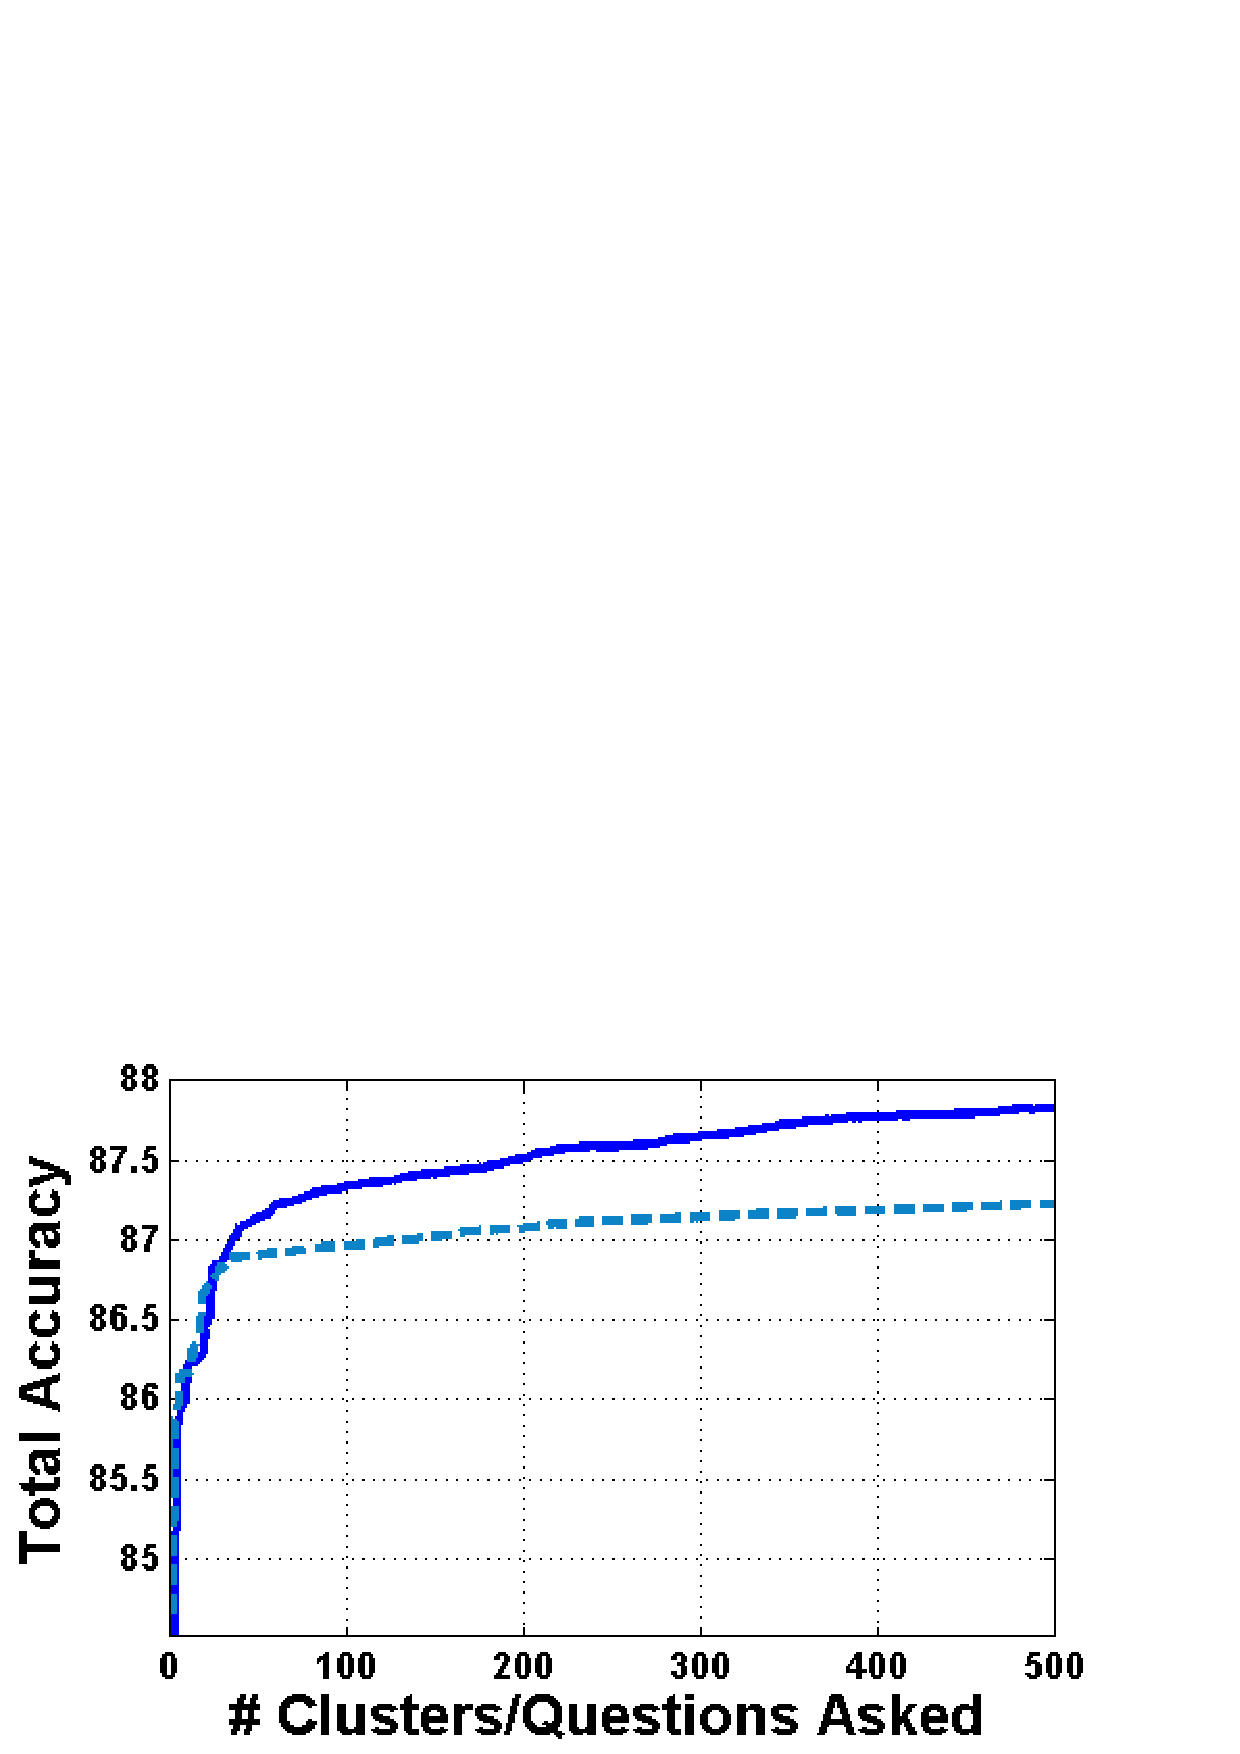
\includegraphics[width=0.22\textwidth]{images/dblp_clustering_compare.png}
        %\label{fig:first2}
    %}
    %\subfigure[PubMed] {
        %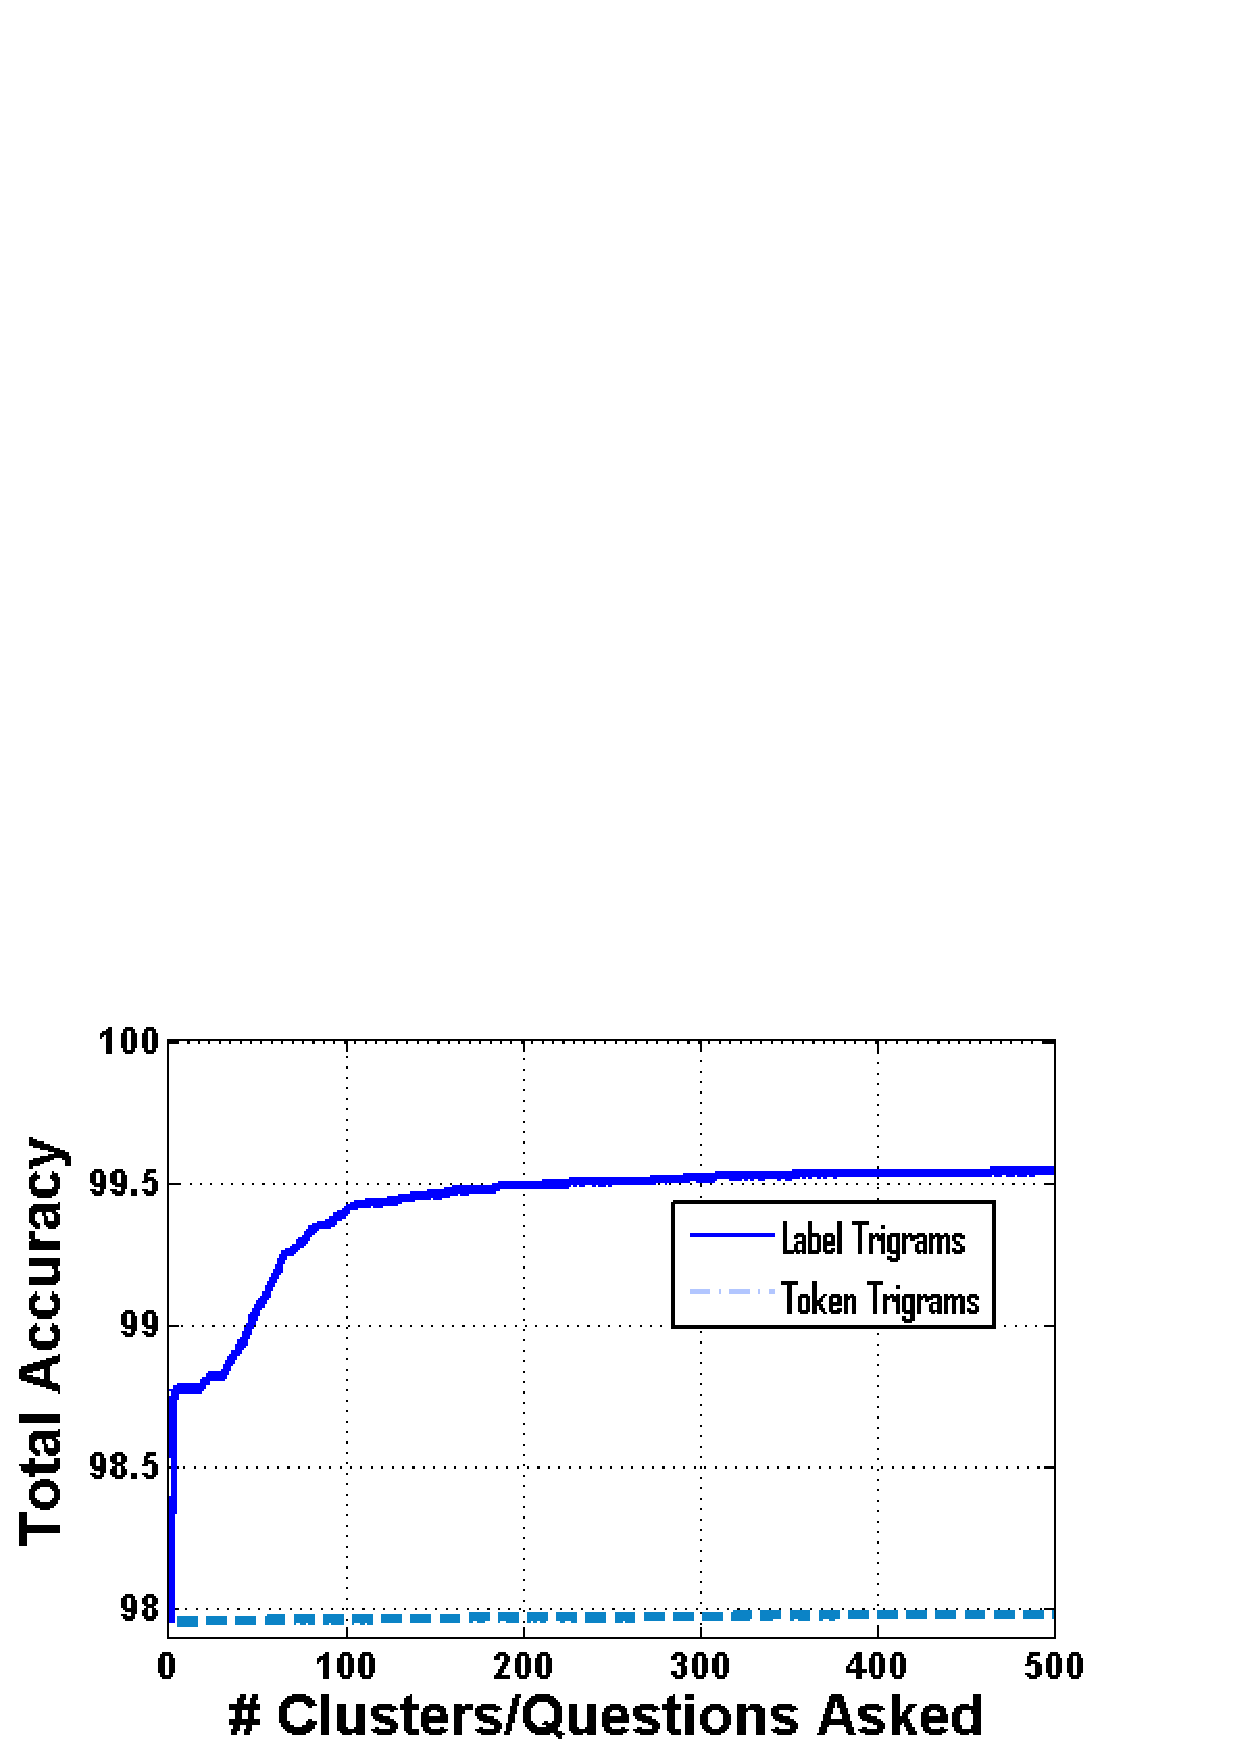
\includegraphics[width=0.22\textwidth]{images/pubmed_clustering_compare2.png}
        %\label{fig:second2}
    %}
    %\caption{Clustering comparison for (a) DBLP and (b) PubMed.  Default seeding is High Entropy and default ranking is Total Entropy.}
    %\label{fig:select2}
%\end{figure}

%In this paper, we proposed two possible functions for selecting a token from each document that maximized information gain.  High Entropy chooses that which has the highest marginal entropy over its labels while Neighborhood Entropy selects the token in the center of the largest 3-window pocket of marginal entropies.  Figures~\ref{fig:first1} \&~\ref{fig:first4} show the effectiveness of both methods when compared to randomly selecting a token.  While comparable in the DBLP set (\ref{fig:first1}), the PubMed set (\ref{fig:first4}) benefits greatly from extracting tokens with the highest Neighborhood Entropy.  Both methods reach accuracy values unobtainable by random selection in fewer than 10 questions.

The results of Figures~\ref{fig:first1} and~\ref{fig:first4} show a marked increase in accuracy using information theoretic techniques after just a few questions compared to selecting at random.  After about 25 questions in the DBLP set, both information theoretic methods produce a 5-fold increase in accuracy compared to random and reduce the overall error by about 15\%.  The initial PubMed accuracy was much better, but still saw a 66\% reduction in error using our selection methods after about 50 questions.  This is significant when considering DBLP contained 36k individual tokens and PubMed 3.3m tokens.  Each question only queries for the label to a single token, so we are seeing large reductions in error querying on significantly small fractions of the data. 

The trigram methods are compared in Figures~\ref{fig:first2} and~\ref{fig:first5}, where label trigrams outperform token trigrams in both data sets.  The knee in the PubMed set is due to several large clusters of similar tokens being selected first.  There are more likely to be misclassification errors using label trigrams, but experiments show the increased coverage outweighs this concern.  Finally, ranking metrics are compared in Figures~\ref{fig:first3} and~\ref{fig:first6}.  The presence of large clustering gives added weight to both methods that take cluster size into account.  Information gain, the sum of a mutual information scores of all tokens in a cluster, takes into account both cluster size and informativeness and excels in both data sets.

%Figures~\ref{fig:first2} \&~\ref{fig:first5} compare the possible clustering algorithms.  For the DBLP set (\ref{fig:first2}), there were zero clustering errors for Same Token and Same Field, and approximately 2\% of citations were clustered incorrectly using the Same Label approach.  The PubMed set (\ref{fig:first5}) also contained no errors for the constrictive Same Token and Same Field, but approximately a 0.2\% error rate for Same Label. Despite introducing additional errors, the gain from clustering a larger number of tokens gives the Same Label mechanism a boost in overall token accuracy.  The gain is most drastic for the PubMed set, where the clusters were much larger.  Same Token and Same Field exhibited minimal clustering as evidenced by the nearly flat lines.

%The final set of selection experiments is shown in Figures~\ref{fig:first3} \&~\ref{fig:first6}.  There is very little difference between the Cluster Size and Total Entropy methods, but both easily eclipse ranking by the representative Highest Token Entropy and reach the same accuracy in 90\% fewer questions for DBLP.  PubMed results are similar, but orders-of-magnitude greater.

%One important comment is that these accuracies are truncated at 500 questions and given a large enough budget one could theoretically reach near-perfect accuracy.


%\begin{figure}
    %\centering
    %\subfigure[DBLP] {
        %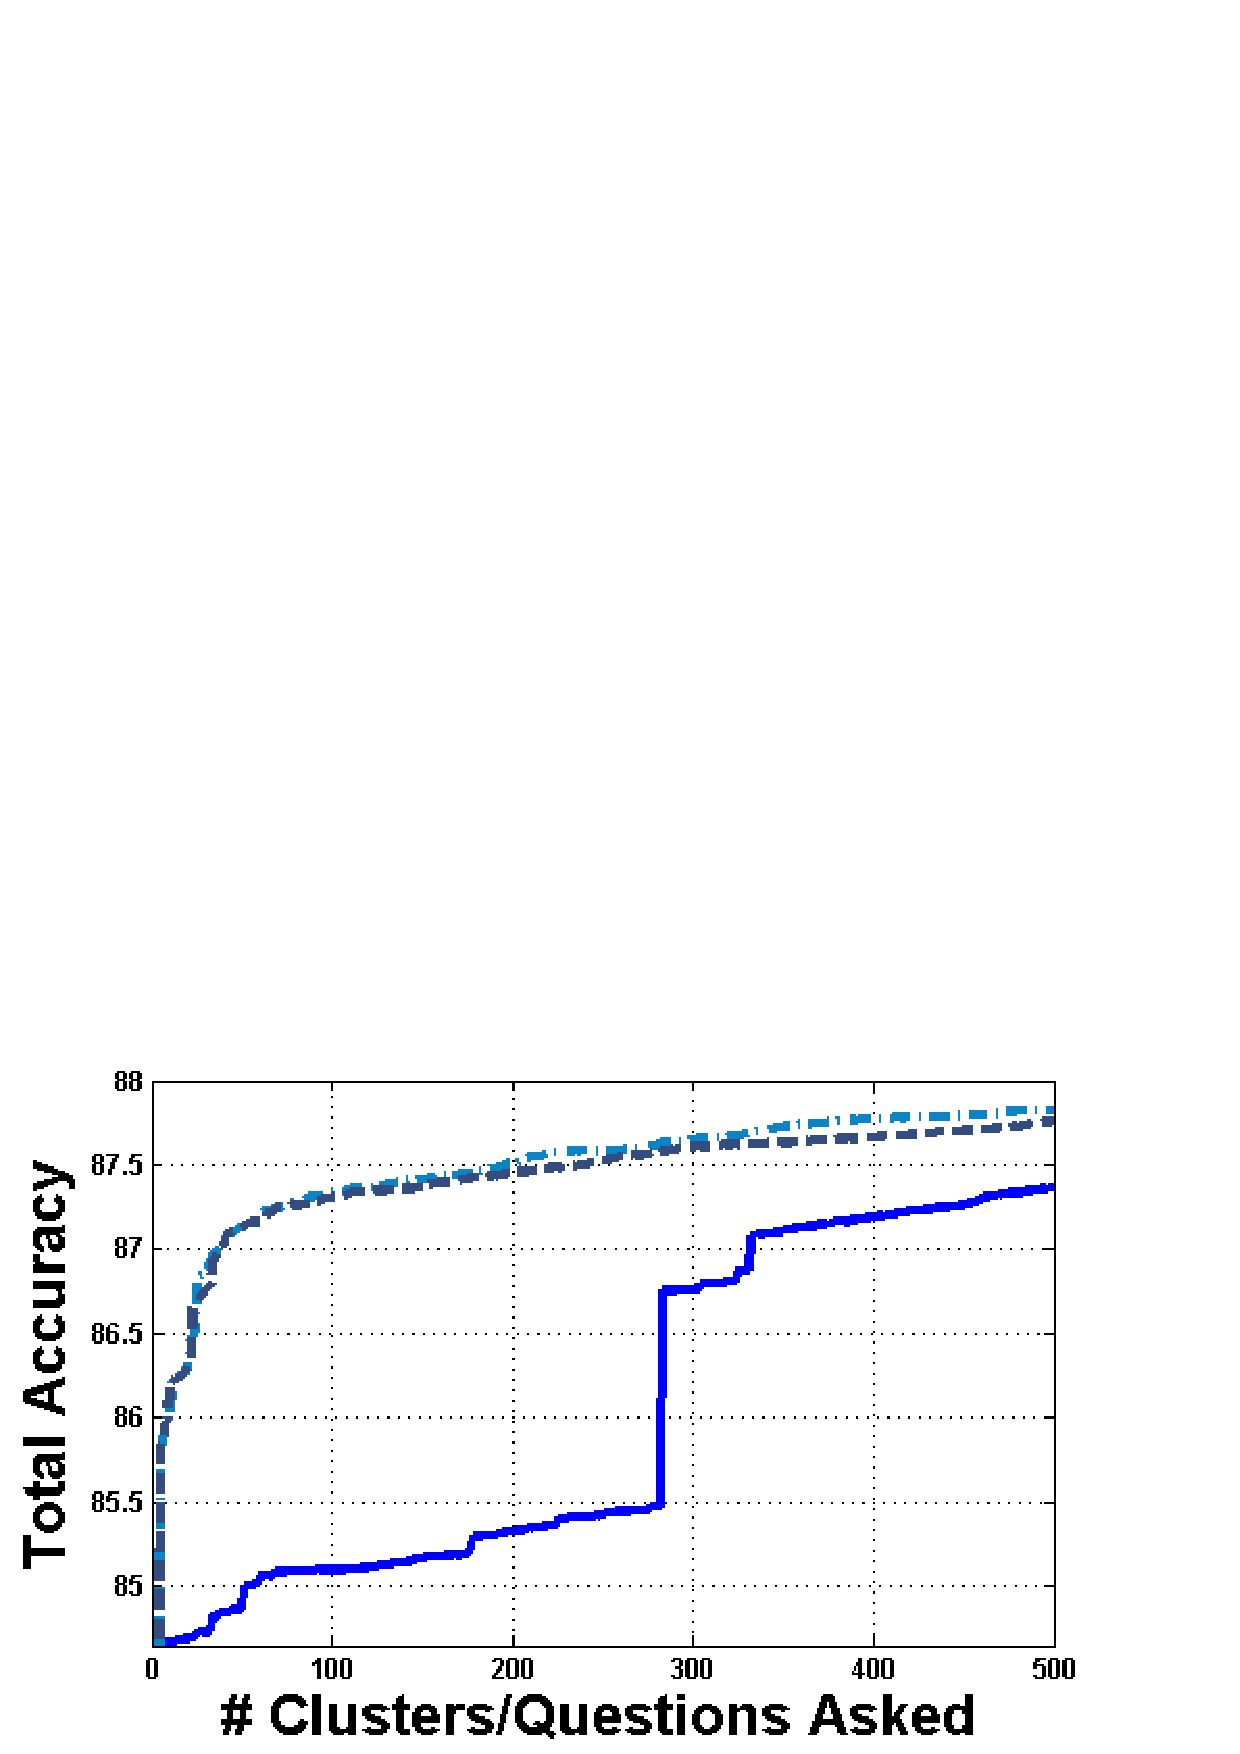
\includegraphics[width=0.22\textwidth]{images/dblp_ranking_compare.png}
    %}
    %\subfigure[PubMed] {
        %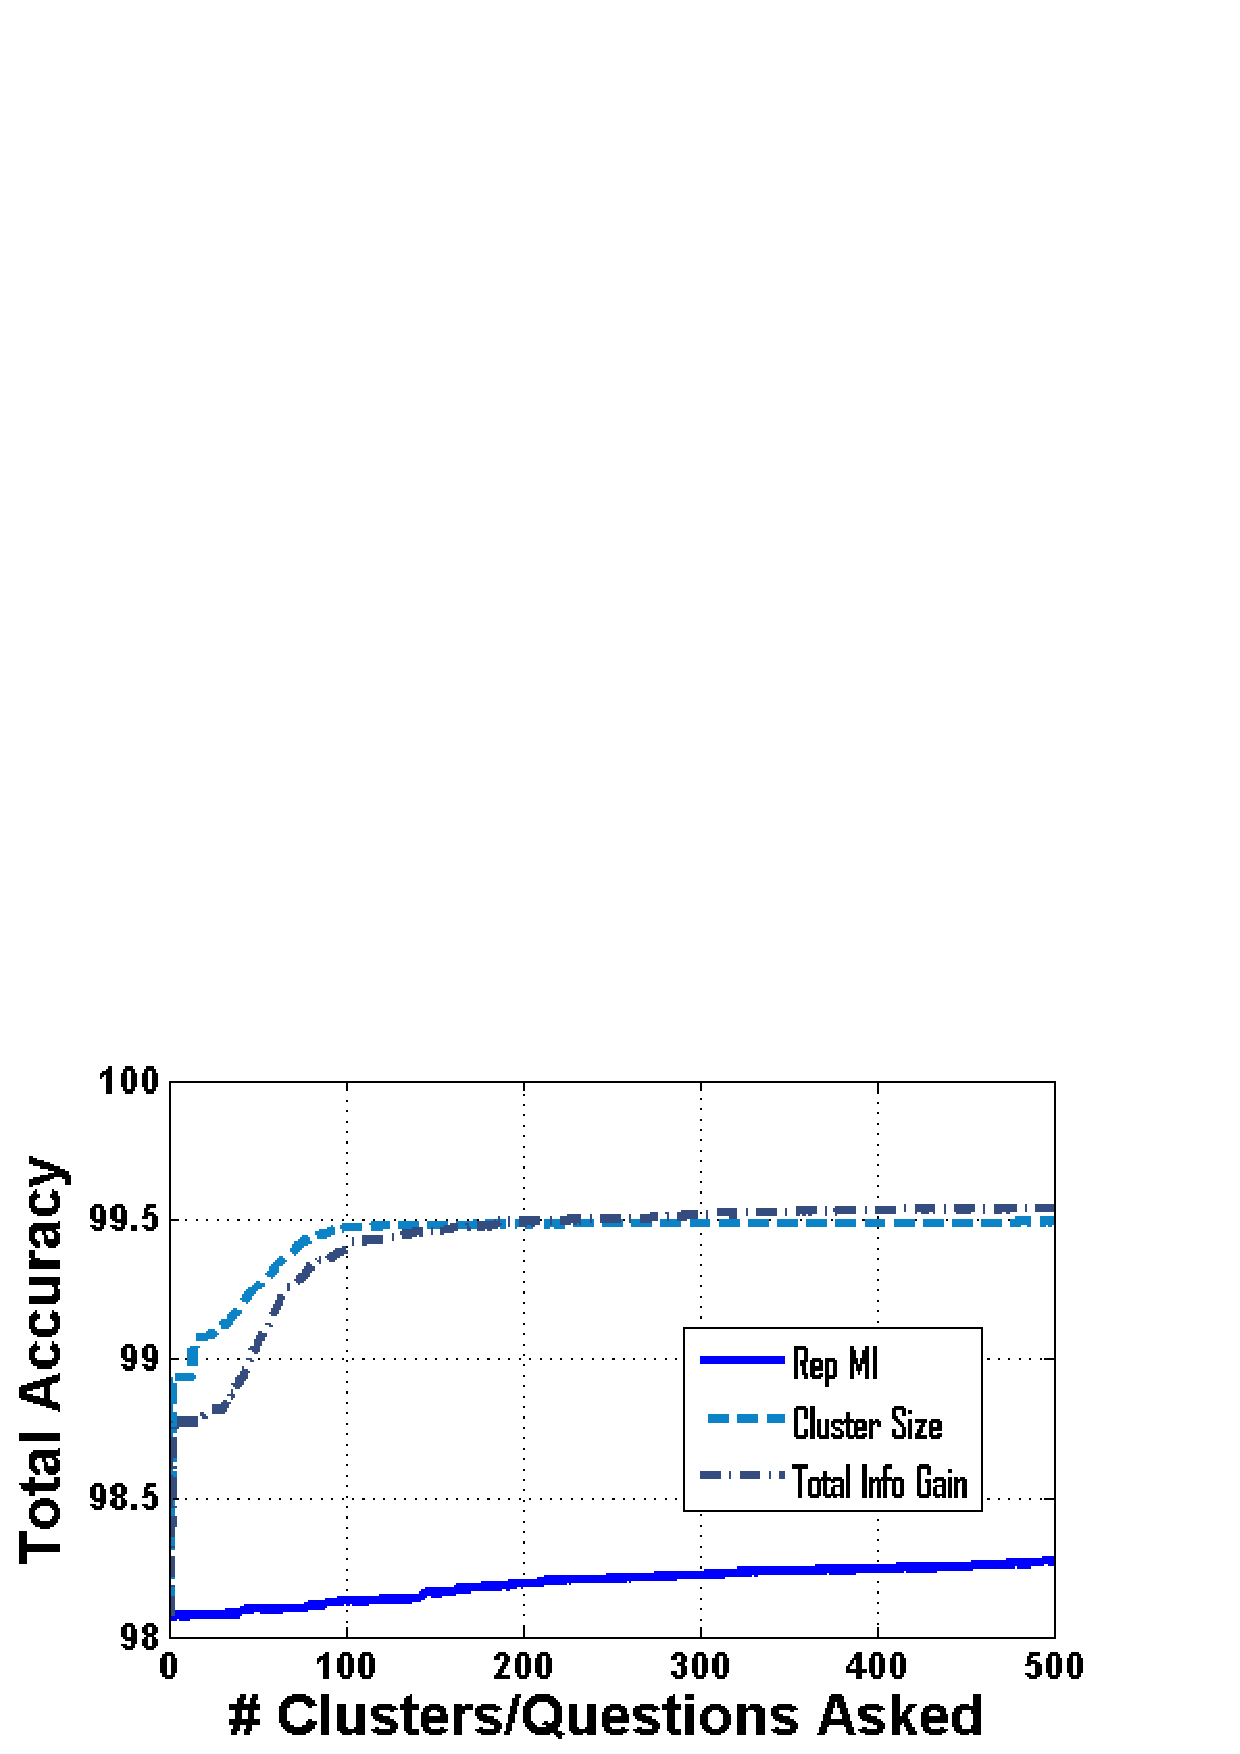
\includegraphics[width=0.22\textwidth]{images/pubmed_ranking_compare2.png}
    %}
    %\caption{Ranking comparison for (a) DBLP and (b) PubMed.  Default seeding is High Entropy and default clustering is Same Label.}
    %\label{fig:select3}
%\end{figure}

\subsection{Integration Experiments}
\begin{figure}[t]
	\centering
	\subfigure[]{        
	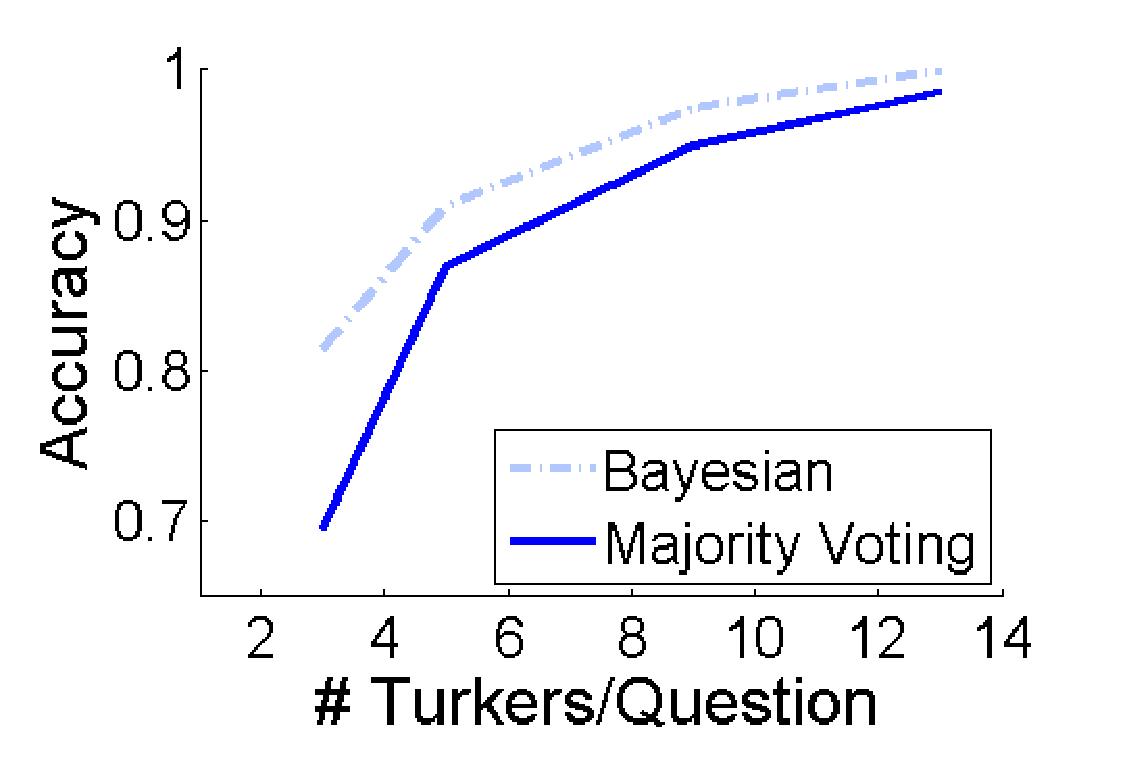
\includegraphics[width=0.47\textwidth]{integration_exp1_numT.eps}
        %\caption{Comparison of integration methods vs. number of Turkers per question for a synthetic set of 500 questions and Turker accuracies drawn from a mean of $0.5$ and standard deviation of $0.3$.}
        \label{fig:integrate1}
	}
\hspace{-4mm}
%\end{figure}
%\begin{figure}[t]
	\subfigure[]{
        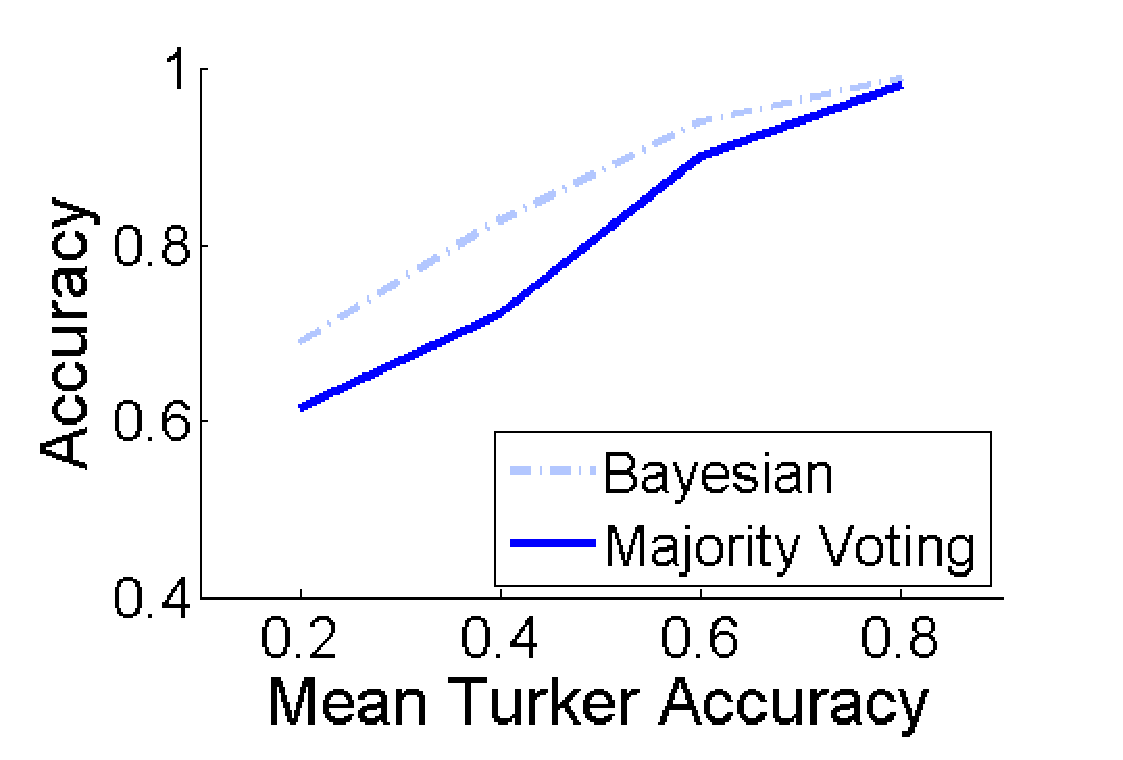
\includegraphics[width=0.47\textwidth]{integration_exp2_meanQ.eps}
        %\caption{Comparison of integration methods vs. average Turker quality for a synthetic set of 500 questions and 5 Turkers per question.}
        \label{fig:integrate2}
	}
	\caption{Comparison of integration methods versus (a) number of Turkers per question and (b) average Turker quality for a synthetic set of 500 questions.  Where not stated the default number of Turkers was 5 and mean accuracy was 0.5.}
%\vspace{-1mm}
\end{figure}

To measure the efficacy of our integration methods, we conducted experiments over both real and synthetically generated data.  The parameters of the synthetic model were listed in Section~\ref{sec:setup} and allowed us to vary both the number of Turkers answering questions and their individual quality values.

\eat{
%Answers received from the crowd have many variables that must be factored into a rigorous justification of any method of combination.  Primarily, we are concerned with measuring how the final combined accuracy is affected both by the number of redundant answers and by the actual quality of the workers.  A set of synthetic responses to real questions were generated in a manner that the allowed the average worker quality to be varied throughout the experiments.
}

\begin{figure}[t]
\subfigure[DBLP] {
    \centering
    \hspace{2.5cm}
%\begin{center}
    \scalebox{1.0}{
    \begin{tabular}{ | l | l |}
    \hline
    Integration Method & Accuracy \\ \hline
    Majority Vote & 97.5 \\ \hline
    Bayesian & 97.5 \\ \hline
    \end{tabular}
    }
\hspace{2.5cm}
%\end{center}
}\\
\subfigure[DBLP-hard] {
%\begin{center}
    \centering
    \hspace{2.5cm}
    \scalebox{1.0}{
    \begin{tabular}{ | l | l |}
    \hline
    Integration Method & Accuracy \\ \hline
    Majority Vote & 75.8 \\ \hline
    Bayesian & 77.3 \\ \hline
    \end{tabular}
    }
\hspace{2.5cm}
%\end{center}
}\\

\subfigure[PubMed] {
%\begin{center}
    \centering
    \hspace{2.5cm}
    \scalebox{1.0}{
    \begin{tabular}{ | l | l |}
    \hline
    Integration Method & Accuracy \\ \hline
    Majority Vote & 14.3 \\ \hline
    Bayesian & 20.9 \\ \hline
    \end{tabular}
    }
    \hspace{2.5cm}
%\end{center}
}
\caption{Amazon Mechanical Turk accuracies for a set of 500 standard (DBLP) and two sets of 500 difficult (DBLP-hard \& PubMed) questions.}
\label{fig:table}
\end{figure}

\eat{
%Workers were automatically generated by selecting a quality value $Q \in [0,1]$ from a Gaussian distribution of standard deviation 0.3 and a mean that varies over the experiment.  Quality values drawn outside the $[0,1]$ range were truncated at the boundary.  Each worker was assigned to a 'HIT', which constituted a set of 10 questions.  The quality level dictated the generation of answers.  In keeping with our assumption of quality, the true label was applied with probability $Q$.  With probability $1-Q$, the answer was drawn from a uniform distribution over the label space.  In this manner we assembled 500 questions answered by 3-13 workers each, with new sets of workers generated every 10 questions.
}

Figure~\ref{fig:integrate1} shows the gain in accuracy that comes with using a probabilistic combination method as opposed to taking a simple majority vote as we increase the number of Turkers answering each question.  The mean worker accuracy is 0.5 in these results and the prior used in the Bayesian method is uniform over a label space of 8 labels.  While both methods increase monotonically as expected, the Bayesian method produces the best results for low redundancy and attains 100\% accuracy before majority voting.

The availability of high or low quality workers is certain to affect the information gathering, so in Figure~\ref{fig:integrate2} we compare the accuracy of answers as we vary the quality.  Variation is achieved by shifting the center of the Gaussian which produces worker quality values.  We initially set it at 0.2 and shifted to a maximum of 0.8.  As before, the Bayesian approach shows that combining probabilistically, even when source accuracies are so low as to be just slightly better than random, produces large gains in answer accuracy. 

%One method of attaining only high quality workers on Amazon Mechanical Turk is to implement a qualification test that workers must pass before they can complete your tasks.  Our experience has shown that while this does lead to more abled workers, the price paid in time can be many times slower.  The results of Figures~\ref{fig:integrate1} and~\ref{fig:integrate2} show that with a better integration method, some of the constraints designed to achieve higher quality may be relaxed without a large decrease in accuracy, key to making \sysName fast, agile, and powerful.

In addition to the synthetically generated Turker data, we performed a set of experiments using our Amazon Mechanical Turk interface.  As described in the introduction to this section, 500 questions from the PubMed and DBLP data sets were provided to Turkers, with both sets containing selected questions to measure the extremes of Turker viability.  The DBLP set contained questions ranked using highest mutual information filtering, label trigram clustering, and total information gain ranking.  It was presented twice to Turkers, the second time being stripped of all punctuation to make the classification problem more difficult.  After integration the maximum likelihood value was compared to the ground truth to determine accuracy.  Figure~\ref{fig:table} shows a comparison for relatively easy DBLP set compared to the harder sets when using either majority voting or Bayesian combination.  The more difficult the question and the lower the quality of the incoming work the larger the increase in benefit with the Bayesian approach, even attaining a nearly 50\% increase in accuracy for the difficult PubMed set.  The main cause for the extreme difficulty in this set was due to a number of ambiguous numerical fields like journal numbers, issue numbers, etc.

%After seeding the PubMed set by highest entropy and clustering by same label, we ranked by highest entropy to produce a set of particularly difficult questions.  While low all around, majority voting is able to produce only 14.3\% accuracy, while Bayesian and Dempster-Shafer achieved 20.9\% and 20.8\% respectively, a gain of almost 50\%.  This is significant because it shows that when the accuracy of the Turkers is fairly good, our methods tend to do no worse than majority voting, but we see the largest gains when Turkers are heavily conflicted or confused.

\begin{figure}[t]
\centering
        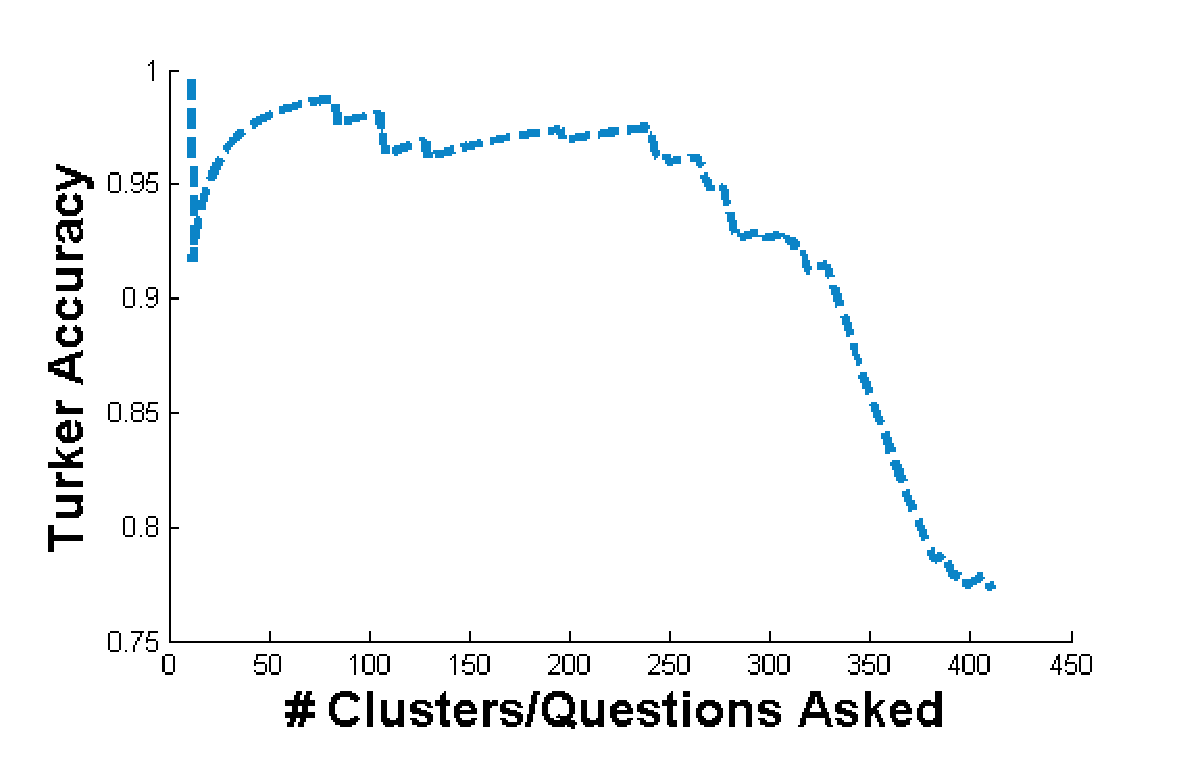
\includegraphics[width=0.95\textwidth]{recall_dblp.eps}
        \caption{Accuracy vs. recall plot for the DBLP-hard data set using probabilistic integration.  If an entropy threshold is set in advance, a high accuracy can be obtained across all accepted answers.}
        \label{fig:recall}
\end{figure}

In addition, one can improve accuracy even further by only accepting those answers for which there is high confidence.  Our probabilistic approach lends itself to a natural confidence indicator in the entropy of the combined distribution.  The trade-off between accuracy and recall is a new functionality compared to deterministic integration which adds flexibility for users to tune the system according to the needs of their application (ie. high accuracy vs. high recall).  Figure~\ref{fig:recall} shows how the accuracy varies for the DBLP-hard set based on how many answers we accept as determined by a confidence threshold.  The initial accuracy was 77\%, but by retaining only the top two-thirds of the answers in this set, we can keep the total accuracy above 90\%.  Previous work~\cite{Sheng:2008:GLI:1401890.1401965} has attempted selectivity by answer entropy.% however, we believe we are the first to probabilistically incorporate Turker reliability into the method.

\eat{
The remaining answers can then be immediately sent back to the crowd for additional querying until their entropy falls below the threshold or a maximum number of answers are received.  This also helps the system identify particularly difficult or troublesome questions.

Originally, we introduced new methods for integration in order to produce a probabilistic result that could provide information on confidence of a crowd combined answer (using its entropy) as well as maintain states of conflict when integrating with additional machine evidence.  What we also find, however, is that we can expect an accuracy boost in addition to new probabilistic features afforded over deterministic integration.  The accuracy gain in the three tables of Figure~\ref{fig:table} compare favorably with the gain observed in Figure~\ref{fig:integrate2}.
}

\noindent\textbf{Summary:} Our experiments show a large savings in cost and gain in accuracy over previous methods.  Selecting those tokens with maximum within-document mutual information and strongest clustering produce an orders-of-magnitude improvement in the number of questions needed compared to random.  Integrating multiple answers probabilistically provides an increase in accuracy by reasoning over Turker uncertainty.  The results in Figure~\ref{fig:table} from real Turker experiments are consistent with those observed synthetically in Figure~\ref{fig:integrate2}.  Finally, probabilistic integration shows promise in providing users with a trade-off between accuracy and recall.

\section{Related Work}
\label{sec:related}
There have been a number of previous attempts at combining humans and machines into a unified data management system, but to our knowledge none that have done it probabilistically.  CrowdDB~\cite{DBLP:conf/sigmod/FranklinKKRX11} utilizes humans to process queries that are either missing from the database or computationally prohibitive to calculate.  The crowd is invoked only if an incoming query contains one of the incomplete values.  In contrast, \sysName operates on batches over a complete, but uncertain database, improving accuracy well in advance of queries.  Qurk~\cite{DBLP:conf/sigmod/MarcusWKMM11} crowdsources workflow operations of the database, such as filtering, aggregating, sorting, and joining, but makes no attempt to optimize the workload between both humans and machines.  AskIt!~\cite{DBLP:conf/icde/BoimGMNPT12} provides a similar goal of "selecting questions" to minimize uncertainty given some budget, however their approach is purely for quality control.  CrowdER~\cite{DBLP:journals/pvldb/WangKFF12} uses a hybrid human-machine system to perform entity resolution.  The machine does an initial course pass over the data and the most likely matching pairs are verified through crowdsourcing.  The primary approach of that work is HIT interface optimization as opposed to the specific question selection and answer integration of ours.  DBLife~\cite{DBLP:conf/cidr/DeRoseSCLBDR07} invites mass collaboration to improve a database seeded by machine learning, but selection is done by humans as needed without any means of automatically identifying likely errors.  There is also no means of doing quality control or redundancy checking if humans introduce erroroneous edits.

\section{Conclusion}
\label{sec:conclusion}
\balance

In this paper we introduce \sysName, a crowd-assisted SML-based IE system that can improve the accuracy of its automated results through a crowdsourced workforce.  Our mutual information-based question selection algorithm produces questions with the largest information gain with a given budget.  Probabilistic answer integration can be achieved using a Bayesian formulation that combines multiple, possibly conflicting Turker answers into a single posterior distribution.  We showed a large improvement in cost, speed, and accuracy over random question selection and standard majority voting combination.  

While we focus on text extraction in the paper, we envision a more general Crowd-Assisted Machine Learning (CAMeL)
system that uses a probabilistic database to efficiently connect and integrate crowdsourcing to improve the imperfect results from SML methods. Many of the core elements developed in \sysName such as uncertainty management, question selection, and uncertain data integration are applicable to other SML-based tasks in CAMeL.



% For one-column wide figures use
%\begin{figure}
% Use the relevant command to insert your figure file.
% For example, with the graphicx package use
%  \includegraphics{example.eps}
% figure caption is below the figure
%\caption{Please write your figure caption here}
%\label{fig:1}       % Give a unique label
%\end{figure}
%
% For two-column wide figures use
%\begin{figure*}
% Use the relevant command to insert your figure file.
% For example, with the graphicx package use
  %\includegraphics[width=0.75\textwidth]{example.eps}
% figure caption is below the figure
%\caption{Please write your figure caption here}
%\label{fig:2}       % Give a unique label
%\end{figure*}
%
% For tables use
\bibliographystyle{ACM-Reference-Format-Journals}
\bibliography{springerBib}

\received{May 2015}{June 2015}{July 2015}


% BibTeX users please use one of
%\bibliographystyle{spbasic}      % basic style, author-year citations
%\bibliographystyle{spmpsci}      % mathematics and physical sciences
%\bibliographystyle{spphys}       % APS-like style for physics
%\bibliography{}   % name your BibTeX data base

% Non-BibTeX users please use


\end{document}

